\chapter{Development} % (fold)
\label{chap:development}

\section*{Reader Guidance} % (fold)
\label{sec:dev_reader_guidance}
This chapter describes in detail the concepts behind the results of this
thesis. In contrast to Chapter~\ref{chap:api}, it is not a matter of defining
the whole API of this library in breadth but of presenting the background and
considerations understandably. \\
The first part of this chapter describes how iterables work in JavaScript and
what a sequence is in the context of this project. Then it shows how to use the
Decorator Pattern to build functions available to all iterables. \\ 
The second part shows how programs can be better structured using approaches
found in functional programming languages. These approaches allow the adoption
of abstract and strong concepts from Haskell to JavaScript. \\ 
The final part is devoted to testing - how to test different functions with
similar requirements safely and why tests based on invariants are helpful.
% section Reader Guidance (end)
\chapter{Iterators in JavaScript} % (fold)
\label{chap:Iterators in JavaScript}
This chapter explains the concept of iterable and iterator objects and points
out features and characteristics of it. The sequence is an implementation of an
iterable. There is a constructor with the same name and a JSDoc type for the
sequence. Many operations can process a sequence. Together with the sequence,
they form the "Sequence library". The following discussion covers challenges
and solutions for creating a robust and user-friendly API.

\section{Iterables in General}
\label{sec:Iterables in General}
In Computer Science, iterators are a popular concept. An iterator provides
access to elements of a data structure. It does not matter if the iterator
accesses a data structure fully kept in memory (like arrays) or if it computes
the elements lazily when queried. In both ways, a function call on the iterator
retrieves the next value. Iterators are an essential part of this work.
Therefore, it is crucial to understand the fundamentals of this concept.

\subsection{Iterable Data Structures in JavaScript}
\label{sub:Iterable data structures in JS}
JavaScript knows two protocols which define how an object can be used for
iteration - the iterable protocol and the iterator
protocol~\cite{mdn_protocols} object, also known as an iterable, represents a
collection of values. A function call on its iterator, gives access to the next
element in the collection - there is no way to access a previous value. Once an
iterator reaches its end, it is considered "used up" - subsequent calls to such
an exhausted iterator won't produce any meaningful results.

\subsubsection{The Iterable Protocol}
\label{subsub:The Iterable Protocol}
In JavaScript, an object is considered as iterable if it contains a property
called |[Symbol.iterator]|. This property signifies that the object is of type
|Iterable<T>|. Invoking the |[Symbol.iterator]| property, creates an
iterator that follows the iterator protocol explained in the following section.
Objects in JavaScript that implement this property can be utilized with
destructuring \footnote{The destructuring assignment syntax is a JavaScript
expression that allows to extract items of iterables into individual
variables.}and |for...of| loops. Listing \ref{lst:iterable_protocols}
showcases an example of an object defining the |[Symbol.iterator]| property.

\begin{lstlisting}[
  style=ES6, 
  caption=Iterable protocol,
  label={lst:iterable_protocols}
  ]
  return {
    [Symbol.iterator]: () => {
      return { next: next }; *'// next is defined in~\ref{lst:iterator_protocol}'*
    }
  }
\end{lstlisting}

\subsubsection{The Iterator Protocol}
\label{subsub:The Iterator Protocol}
Invoking the |[Symbol.iterator]| property obtains an iterator object
complying to the iterator protocol. It must implement a function |next|, which
defines how and which values are returned when iterating. Each iteration on an
iterator calls this function. |next| returns an object, which must
include two properties: |value| and |done|. The property |value|
contains the current value of the iteration, while |done| represents the
information on whether the end of the iterator has been reached. The following
code \ref{lst:iterator_protocol} shows a simple implementation of it. Each call
on |next| returns an object with the |value 1|. |done| is always |false| -
hence the iterator never ends. 

\begin{lstlisting}[
  style=ES6, caption=Iterator protocol,
  label={lst:iterator_protocol}
  ]
  const next = () => {
    return { done: false, value: 1 };
  };
\end{lstlisting}

\subsubsection{Creating Iterables}
\label{subsub:Creating Iterables}
By combining these two protocols, the result could look like listing
\ref{lst:protocols}. The constructor |InfiniteOnesIterable| on
line~\ref{line:ctor_infiniteones} wraps the two
previously defined implementations. This constructor therefore constructs
iterable objects. Since the return value is a number, this is an
iterable of type |Iterable<Number>|.

\begin{lstlisting}[
  style=ES6, caption=Iterable and iterator protocol,
  label={lst:protocols}
  ]
const InfiniteOnesIterable = () => {*'\label{line:ctor_infiniteones}'*
  const next = () => ({ done: false, value: 1 });

  return {
    [Symbol.iterator]: () => ({ next })
  }
};

const [one, anotherOne, andOneAgain] = InfiniteOnesIterable();*'\label{line:infiniteones_destructuring}'*

for (const _one of InfiniteOnesIterable()) { 
  // hangs forever, since done is always false
}*'\label{line:infiniteones_forof}'*
\end{lstlisting}

Because objects created by |InfiniteOnesIterable| adhere to the JS iteration
protocols, it is possible to use language features like |for..of| and
destructuring to process these objects as shown on
line~\ref{line:infiniteones_destructuring} to~\ref{line:infiniteones_forof}.
However, beware of this case. This would lead to an infinite loop because the
property |done| never becomes |true|. Therefore, the iteration never ends. This
work shows finite iterables later. For now, the focus is on the protocols.
Therefore, this example is sufficient at this point.
\newline
Such protocols make it possible to build customized iterables and
collections. This opens new possibilities. Various programming tasks can have 
different, more straightforward solving approaches in a more declarative way to
write.
There are already some JavaScript iterables present. Arrays and
|HTMLCollection|s are probably the most prominent of these.

\subsection{Types of Iterables}
\label{sub:Types of Iterables}
JavaScript distinguishes between iterables and iterators. These
protocols also have their corresponding types. Listing \ref{lst:iterable_types}
shows an excerpt of them:

\begin{lstlisting}[
  style=ES6, caption=Types of iterables,
  label={lst:iterable_types}
  ]
// lib.es2015.iterable.d.ts

interface Iterable<T> {*'\label{line:start_iteration_types}'*
    [Symbol.iterator](): Iterator<T>;
}

interface Iterator<T, TReturn = any, TNext = undefined> {
  next(...args: [] | [TNext]): IteratorResult<T, TReturn>;
    return?(value?: TReturn): IteratorResult<T, TReturn>;
    throw?(e?: any): IteratorResult<T, TReturn>;
}*'\label{line:end_iteration_types}'*

type IteratorResult<T, TReturn = any> = IteratorYieldResult<T> *'\label{line:start_iteration_result_types}'*
                                      | IteratorReturnResult<TReturn>;


interface IteratorYieldResult<TYield> {
    done?: false;
    value: TYield;
}

interface IteratorReturnResult<TReturn> {
    done: true;*'\label{line:iteration_return_result_done}'*
    value: TReturn;
} *'\label{line:end_iteration_result_types}'*
\end{lstlisting}

\begin{itemize}
  \item{Line~\ref{line:start_iteration_types}~-~\ref{line:end_iteration_types}: 
      An |Iterable| is of type |Iterable<T>|, whereas the object returned by the property
      |[Symbol.Iterator]| is of type |Iterator<...>|. An |Iterator| requires having a property |next|. 
      This is the function that returns values when iterating. These values must be 
      of type |IteratorResult<...>.|
    }
  \item{Line~\ref{line:start_iteration_result_types}~-~\ref{line:end_iteration_result_types}:
      |IteratorResult<...>| itself is defined to return an 
      object of type |IteratorReturnResult<...>|, which either is of type
      |IteratorYieldResult| or |IteratorReturnResult|. This object contains the actual 
      values we want to work with.}
\end{itemize}

Section~\ref{subsub:Stateful Decorating} explains the reason for this nested
architecture of the JS iteration protocols.

\subsubsection{Closer Look to IteratorReturnResult}
\label{subsub:Closer look to IteratorReturnResult}
When iterating an iterable, the returned elements are of type
|IteratorYieldResult<T>|. Calling the function |next| on an exhausted iterator
returns an element of type |IteratorReturnResult<TReturn>|. This ensures that
|done| is set to |true|, as can be seen on
line~\ref{line:iteration_return_result_done} in
listing~\ref{lst:iterable_types}.

\subsection{Illustration of the JS Iteration Protocol}
\label{sub:Illustration of the JS Iteration Protocol}
Listing~\ref{lst:example_js_iteration_protocol} illustrates the behavior of the
JS iteration protocols more clearly using a sample scenario. Since array is an
iterable, we can use it for the following demonstration:

\begin{lstlisting}[
  style=ES6, 
  caption=Example: JS Iteration Protocol,
  label={lst:example_js_iteration_protocol}
  ]
// array including two values, 0 and 1
const list = [0, 1];
const iterator = list[Symbol.iterator]();*'\label{line:illustraion_create_iterator}'*

iterator.next(); // returns { done: false, value: 0 }
iterator.next(); // returns { done: false, value: 1 }
iterator.next(); // returns { done: true,  value: undefined }
iterator.next(); // returns { done: true,  value: undefined }
\end{lstlisting}

On line~\ref{line:illustraion_create_iterator}, invoking |[Symbol.iterator]|
returns the iterator of the iterable |list|. 
After that, we call |next| four times directly on the iterator. Since the
iterable contains only two elements, the third and fourth call on |next|
returns an object of type |IteratorReturnResult<TReturn>|. Thereby, |done| is
|true| and |value| is |undefined|. \\
By using |for...of| and destructuring, an iterable would stop iterating after
the second call. This means an |for...of| loop runs until the property |done|
is set to |true|.

\section{Sequence: An iterable Series of Values}
\label{sec:Sequence: A Series of Values}
In Computer Science, naming elements accurately poses a significant challenge 
when aiming to develop sustainable and robust code. We decided to name series
of data a "sequence". It has been influenced by several factors:

\begin{itemize}
  \item Sequences are not conventional lists known from other programming
    languages.
\item The name sequence is already known from mathematics.
\item Giving this data structure a more familiar name, for example "list",
  leads to wrong assumptions. 
\end{itemize}
What distinguishes the object generated by the sequence from the conventional
list is that a sequence generates its values when they are requested.
Therefore, it needs almost no memory. At the same time, you have the impression
that you are dealing with a vast amount of data. So the constructor |Sequence|
emerged, which generates such a series of data.

\subsection{Components of a Sequence}
\label{sub:Components of a Sequence}
Defining a sequence requires specifying three essential points:
\begin{enumerate}
  \item{A fixed starting value for the sequence} 
  \item{A function that determines whether the sequence should generate
    further values} 
  \item{A function to calculate the next value based on its predecessor} 
\end{enumerate}
Listing \ref{lst:sequence} on line~\ref{line:seq_args} shows the passing of
these three elements as arguments to the constructor. To keep the focus on the
core elements of the sequence, some functionality in listing \ref{lst:sequence}
is omitted and discussed later. The |next| function, explained by
section~\ref{subsub:The Iterator Protocol}, is on
lines~\ref{line:start_protocol}~-~\ref{line:end_protocol}. It contains the
logic to return the next value in an iteration. First, it uses |whileFunction|
to check if the sequence has finished. If this is not the case, the
|incrementFunction| calculates the next element, which afterward will be
returned.

\begin{lstlisting}[
  style=ES6, 
  caption=Parts of Sequence,
  label={lst:sequence}
  ]
// Sequence.js
const Sequence = (start, whileFunction, incrementFunction) => {*'\label{line:seq_args}'*

  const iterator = () => {
    let value = start;
    /**
     * @template _T_
     * Returns the next iteration of this iterable object.
     * @returns { IteratorResult<_T_, _T_> }
     */
    const next = () => {*'\label{line:start_protocol}'*
      const current = value;
      const done = !whileFunction(current);
      if (!done) value = incrementFunction(value);
      return { done, value: current };*'\label{line:end_protocol}'*
    };

    return { next };
  };

  return  /* omitted */;
};
\end{lstlisting}

\subsection{Using a Sequence}
\label{sub:Using a Sequence}
Listing \ref{lst:even-sequence} shows the definition of a sequence of even 
numbers smaller than ten and how to use it. 
\begin{lstlisting}[
  style=ES6, 
  caption=Sequence of even numbers,
  label={lst:even-sequence}
  ]
const startValue        = 0;
const whileFunction     = x => x < 10;
const incrementFunction = x => x + 2;

const seq = Sequence(startValue, whileFunction, incrementFunction);

for (const elem of seq) {
  console.log(elem);
}
// => Logs '0, 2, 4, 6, 8' *'\label{line:demo_output}'*
\end{lstlisting}

The |for..of| loop iterates over the sequence until |done| becomes |true|.
Meanwhile, |console.log| writes the elements to the console.
Line~\ref{line:demo_output} shows the output produced.


\subsection{Range - A Real-World Example}
\label{sub:Range - A Real-World Example}
When considering sequences, a common requirement is to generate a series of
numbers, often with a specified starting point, an end value, and adjustable
increments. This is a classic definition of implementing a range.
Ranges are built into many programming languages such as
Haskell~\cite{haskell_list}, Python~\cite{python_range} or
Kotlin~\cite{kotlin_ranges}. Therefore, we also implemented a range using the
sequence constructor. 

Listing~\ref{lst:range_haskell} shows the construction of a range in Haskell.
\begin{lstlisting}[
  style=Haskell,
  caption=Range in Haskell,
  label={lst:range_haskell}
]
ghci> r = [1..10] -- contains the numbers from 1 up to 10.
ghci> r
[1,2,3,4,5,6,7,8,9,10]
ghci> r = [1..] -- contains an infinite range
\end{lstlisting}

Listing~\ref{lst:kolibri_range} demonstrates different ways to initialize a
range using the Sequence library.

\begin{lstlisting}[
  style=ES6, 
  caption=Kolibri toolkit Range,
  label={lst:kolibri_range}
  ]
 const range               = Range(3);
 const [five, three, one]  = Range(1, 5, -2);
 const [three, four, five] = Range(5, 3);
\end{lstlisting}

\subsubsection{What can a Range be used for?}
\label{subsub:What can a Range be used for?}
Ranges offer efficient processing of sequences of almost any size, consuming
minimal memory resources. As a result, they serve as excellent foundational
components for larger structures. They can be utilized for lazily generating
numbers or executing a specific action several times.

\subsubsection{The Boundaries}
\label{subsub:The Boundaries}
Built-in ranges are commonly available in various programming languages - the
concept of ranges is therefore well-known. However, it is worth noting that not
all languages handle range boundaries similarly. For instance, Kotlin and
Haskell consider both boundaries inclusive. Thus, a range from 1 to 3 in these
languages would include the elements 1, 2, and 3. On the other hand, in Python,
only the lower limit is inclusive. Therefore, the boundaries must be set as 1
and 4 to create an equivalent range in Python. Since it seems more intuitive to
have both borders inclusive, the range for Kolibri toolkit works accordingly.

\subsubsection{Implementation}
\label{subsub:Implementation}
A range uses a sequence under the hood. Helper functions analyze the passed
parameters and, if necessary, reorder them to return the desired sequence.
Listing~\ref{lst:impl_range} shows the main part of the implementation of the
range:

\begin{lstlisting}[
  style=ES6, 
  caption=Implementation of the Range,
  label={lst:impl_range}
  ]
/**
 * @constructor
 * @pure
 * @param { !Number } firstBoundary  - the first boundary of the range
 * @param { Number }  secondBoundary - optional second boundary of the Range
 * @param { Number }  step - size of a step, processed during each iteration
 * @returns SequenceType<Number>
 */
const Range = (fstBoundary, sndBoundary = 0, step = 1) => {
  const stepIsNegative = 0 > step;
  const [left, right] = normalize(fstBoundary, sndBoundary, stepIsNegative);

  return Sequence(
    left,                                                // start value
    value => hasReachedEnd(stepIsNegative, value, right),// while function
    value => value + step                                // increment function
    );
};
\end{lstlisting}

While closely examining the features of a range, we will also cover the functions
|normalize| and |hasReachedEnd| to explain them in more detail.

\subsubsection{Features}
\label{subsub:Features}

\begin{itemize}
  \item \textbf{Parametrization:} The range takes 1–3 parameters. The
    parameters specify the lower limit, the upper limit, and the step size. If
  not all parameters are set, the range uses suitable default values.
\item \textbf{Interchangeable boundaries:} The order of the lower and the upper
  limit is Interchangeable when creating a new range.
\item \textbf{Negative boundaries and step:} The boundaries and the step size
  of the range can be positive or negative integers.
\end{itemize}

\subsubsection{Normalization of the Boundaries}
\label{subsub:Normalization of the Boundaries}
To ensure flexibility, the range provides the interchangeability of boundaries
and the option for positive or negative step values. Initially, the range
boundaries are normalized based on the step value. This normalization
determines which boundary will contain the first generated number and which
will represent the last number.
The following figure~\ref{fig:norm-flowchart} explains the process in detail.

\begin{figure}[H]
    \centering
    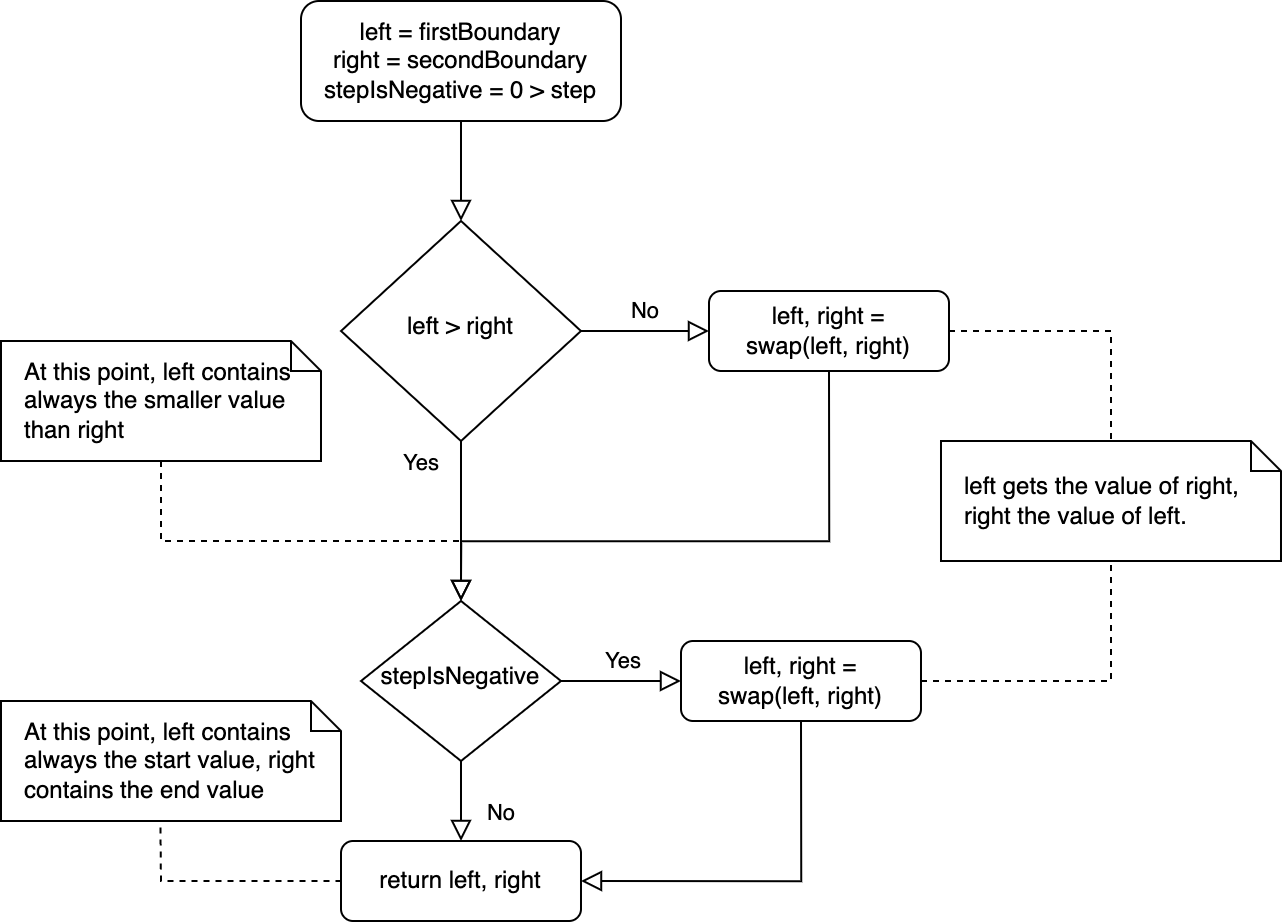
\includegraphics[width=0.9\textwidth]{mainmatter/pictures/boundary-normalization.png}
    \caption{Normalization Flow-Chart diagram}
    \label{fig:norm-flowchart}
\end{figure}

\subsubsection{The End of a Range}
\label{subsub:The End of a Range}
The |hasReachedEnd| function detects the end of the range and defines the
|untilFunction| of the underlying sequence. Listing~\ref{lst:impl_hasReachedEnd}
shows the implementation of the function:

\begin{lstlisting}[
  style=ES6, 
  caption=hasReachedEnd implementation,
  label={lst:impl_hasReachedEnd}
  ]
/**
 * Determines if the end of the range is reached.
 * @param   { Boolean } stepIsNegative
 * @param   { Number }  next - the current element of the range
 * @param   { Number }  end  - the last value of the range
 * @returns { boolean }
 */
const hasReachedEnd = (stepIsNegative, next, end) =>
    stepIsNegative ? next < end : next > end;
\end{lstlisting}

The function must be able to distinguish between two different cases:

\begin{itemize}
  \item If the step size is a negative, the range counts from top to bottom:
    The range reached its end as soon as next is smaller than right.
  \item If the step size is positive, the range counts from bottom to top: The
  range reached its end as soon as next is larger than right.
\end{itemize}

\subsubsection{Some Restrictions of Using a Range}
\label{subsub:Some Restrictions of Using a Range}
When using the range, one has to pay attention to the contract:
\begin{itemize}
\item End value may not be reached exactly, but will never be exceeded.
  \item Zero step size leads to infinite loops, returning always the same values.
  \item Only values that behave correctly with respect to addition and size
    comparison may be passed as arguments.
\end{itemize}


\subsubsection{Using a Range}
\label{subsub:Using a Range}
Following listing~\ref{lst:range_examples} demonstrates various ways to
construct a range.

\begin{lstlisting}[
  style=ES6, 
  caption=Range examples,
  label={lst:range_examples}
  ]
// typical cases
for (const value of Range(3)) { console.log(value); }
// => Logs '0, 1, 2, 3'

for (const value of Range(2,3)) { console.log(value); }
// => Logs '2, 3'

// lower and upper boundaries interchanged
for (const value of Range(3,2,1)) { console.log(value); }
// => Logs '2, 3'

// negative step size
for (const value of Range(4,6,-2)) { console.log(value); }
// => Logs '6, 4'

for (const value of Range(6,4,-2)) { console.log(value); }
// => Logs '6, 4'

// range with negatgive boundary
for (const value of Range(0,-2,-1)) { console.log(value); }
// => Logs '0, -1, -1'
\end{lstlisting}

\section{Iterables Everywhere}
\label{sec:Iterables Everywhere}
The JS iteration protocols are suitable for a wide variety of data structures.
With the sequence library defining many operations for iterables, it makes
sense to make more objects iterable. For example, the Kolibri Web UI toolkit
defines the immutable data structure "pair", for which there are noteworthy
applications if it is iterable. 
\subsection{Making immutable Data Structures iterable}
\label{sub:Making immutable Data Structures iterable}
Listing~\ref{lst:pair_non_iterable} defines the type pair and shows its usage:
\begin{lstlisting}[
  style=ES6, 
  caption=Immutable Pair,
  label={lst:pair_non_iterable}
  ]
/** *'\label{line:start_pair_type}'*
 * @typedef PairType
 * @type {  <_T_, _U_>
 *          (x: _T_)
 *       => (y: _U_)
 *       => (s: PairSelectorType<_T_, _U_>) => ( _T_ | _U_ ) 
 *      }
 */ *'\label{line:end_pair_type}'*
const Pair = x => y => selector => selector(x)(y);

const pair = Pair(1)(2);

const one  = pair(fst);*'\label{line:fst_pair}'*
const two  = pair(snd);*'\label{line:snd_pair}'*

console.log(one + " " + two);
// => Logs '1 2'
\end{lstlisting}

The only way to make a pair immutable is to build it using functions. The type 
signature on line~\ref{line:start_pair_type}~-~\ref{line:end_pair_type} shows 
that the first two arguments are arbitrary values. Pair stores these two values
in its closure scope, the only scope in JavaScript which can not be changed in
any way from the outside.
Selector functions named |fst| on line~\ref{line:fst_pair} and |snd| on 
line~\ref{line:snd_pair} grant access to these values. However, pair offers
no way to modify these values. Listing~\ref{lst:pair_non_iterable} shows that
handling a pair can be tedious. It would be great to use the built-in
JavaScript language features to access the content of a pair.

\subsubsection{Iterable Pair}
\label{subsub:Iterable Pair}
Listing~\ref{lst:pair_iterable} demonstrates the implementation of an iterable 
pair. Still, pair operates only with functions. However, it additionally defines the
|[Symbol.iterator]| property:

\begin{lstlisting}[
  style=ES6, 
  caption=Iterable Pair,
  label={lst:pair_iterable}
  ]
const Pair = x => y => {
  /**
   * @template _T_, _U_
   * @type { PairSelectorType<_T_,_U_> }
   */
  const pair = selector => selector(x)(y);

  pair[Symbol.iterator] = () => [x,y][Symbol.iterator]();*'\label{line:pair_symbol_iterator}'*

  return pair;
};
\end{lstlisting}

Line~\ref{line:pair_symbol_iterator} shows that 
this property defines a function, which only returns the |[Symbol.iterator]|
property of array. The array stores the values of the pair. With that, pairs
are now iterable. Listing~\ref{lst:handling_pair_iterable} shows the usage of
such an iterable pair. Line~\ref{line:pair_destructuring} shows the
deconstruction of a pair in the same way as an array. This access option is
more convenient than in listing~\ref{lst:pair_non_iterable}.
Line~\ref{line:show_pair} demonstrates the usage of operations from the Sequence
library alongside a pair. |show| converts an iterable into a string, analogous
to how |toString| works.

\begin{lstlisting}[
  style=ES6, 
  caption=Working with iterable Pairs,
  label={lst:handling_pair_iterable}
  ]
const pair = Pair(1)(2);

const [one, two] = pair;*'\label{line:pair_destructuring}'*

console.log(show(pair));*'\label{line:show_pair}'*
// => Logs '[1,2]'
\end{lstlisting}

This has significant advantages because it is now possible to process different 
collections with the same abstractions. Therefore, the motivation is great to 
make all collections iterable.

% chapter Iterators in JavaScript (end)

\section{Decorating Sequences}
\label{sec:Decorating Sequences}
This chapter explores how to modify Sequences by implementing the Decorator 
Pattern and effectively managing Sequence state. And then we will discover 
powerful techniques to enhance Sequence functionality and manipulate data.

\subsection{Decorator Pattern}
\label{sub:Decorator Pattern}
Let us look at the Decorator Pattern~\cite[p.~226]{gang_of_four_depa} to understand the content of the 
following sections. In object-oriented programming, the Decorator Pattern is a 
widely used concept. An object decorates another, as the name implies. As a 
result, an outer object holds an inner object, while both implement the same 
interface. The outer object forwards requests to the inner one. This enables
the outer to modify (decorate) the behavior of the inner. 
Figure \ref{fig:seq_diagramm} shows how a decorator forwards the receiving calls and 
transfers the answer back to the client.

% TODO: replace
\begin{figure}[H]
    \centering
    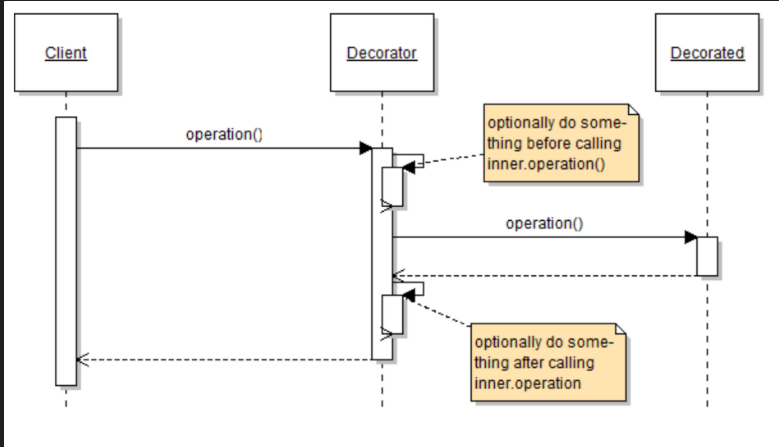
\includegraphics[width=0.8\textwidth]{./mainmatter/pictures/decorator_sequence_diagramm.png}
    \caption{Decorator Patter Sequence Diagram}
    \label{fig:seq_diagramm}
\end{figure}

The Decorator Pattern is often used in object-oriented programming languages 
because of its ability to add functionality to an object at runtime. It is also 
possible to add extended functionality to a single class object. In the 
following, we will see how to exploit this to manipulate and change an Iterable.

\subsection{Processing Sequences}
\label{sec:Processing Sequences}
This section explains how the Sequence Library uses the Decorator pattern.
In the following, the |map| implementation demonstrates the implementation of it. 

\subsubsection{Processing Iteratbles with Functions}
\label{subsub:Processing Iterables with Functions}
In the following, |map| serves as a representative for any function of the
Sequence Library. We call such functions in the following operators,
according to the package they are in.
Listing~\ref{lst:impl_map} shows how |map| processes a Sequence. The
implementation use the Decorator approach just mentioned. |map| decorates a
|Sequence| on line~\ref{line:obj_mapped}.
\newline
On line~\ref{line:args}, the function signature shows that a client can invoke 
|map| with two arguments:

\begin{enumerate}
  \item{A mapper-function capable of processing an element of an |Iterable|}
  \item{An |Iterable|}
\end{enumerate}

An iterable must adhere to the JS iteration protocol 
outlined in Section~\ref{subsub:The Iterable Protocol}. Therefore, |map| can 
process Sequences, Arrays, or any other iterable. 

\begin{lstlisting}[
  style=ES6, 
  caption=Implementation of map,
  label={lst:impl_map}
  ]
const map = mapper => iterable => { *'\label{line:args}'*
*'\label{line:state_iterable}'*
const mapIterator = () => {
   const inner = iteratorOf(iterable);*'\label{line:state_iterator}'*
   let mappedValue;
 
   const next = () => {
     const { done, value } = inner.next();*'\label{line:inner_next}'*
     if (!done) mappedValue = mapper(value);
 
     return { /**@type boolean */ done, value: mappedValue }
   };
 
   return { next };
  };
 
  return createMonadicSequence(mapIterator);
};

const sequence = Sequence(0, x => x < 10, x => x++);*'\label{line:seq_definition}'*
const mapped   = map(x => x * 2)(sequence);*'\label{line:obj_mapped}'*
\end{lstlisting}

Because |map| decorates iterables, |map| also returns an object adhering JS
iteration protocols. 
We define this object on line~\ref{line:obj_mapped} as |mapped|. 
Consequently, |map| also has a next function. Since the JS iteration protocol 
specifies only this single function, it is the only one that must be externally 
callable. The object |mapped| forwards function calls on |next| to the
inner function |next|, on line~\ref{line:inner_next}. The |mapper| function then 
processes the result and returns it. so |map| decorates the function |next| of
the inner |Iterable|.

\subsection{Benefits of the Decorator Approach}
\label{sub:Benefits of the Decorator Approach}
This section discusses the benefits and consequences of using the Decorator 
Pattern to implement the Sequence Library. We start with the fact that functions 
stand-alone, then discuss the options for managing State.

\subsubsection{Stand-alone Functions}
\label{subsub:Standalone Functions}
In an object-oriented approach, the |Sequence| object would provide a function
|map|. Therefore, such operators are available by using dot notation,
similar to Java implements the Stream API \cite{java_stream}. 
However, with the approach of providing independent functions, there 
are three significant advantages:

\begin{enumerate}
  \item {Strict adherence to the open-close principle~\cite[p.~3]{eilebrecht_patterns_2019}. Changes to an operator do
      not affect the implementation of Sequence. Also, extensions to the 
      Sequence Library do not affect existing code.
    }
  \item{Adherence to the single responsibility approach. The Sequence 
      constructor has only the task of creating a sequence. Mapping the
    elements of a sequence is not its responsibility.
  }
  \item{Easy scalability is guaranteed. It is very straightforward to add new 
    functionality from the outside.
  }
\end{enumerate}

Additionally, the |operators| implement their arguments in a curried-style, passing the
receiver at the last position allows the use of eta-reduction in many situations. 
More about this later in the paper.

\subsubsection{Stateful Decorating}
\label{subsub:Stateful Decorating}
A state is present as soon as operators decorate iterables or implement 
additional functionalities. This chapter explores the implementation of state
within operators and the implications it involves.

There are two valid possibilities for including state.
The first Scenario places the state into the closure scope to the surrounding 
operator of the iterator. The second Scenario implements the state into the 
closure scope of the iterator. In both variants, it is crucial to ensure that 
the underlying object remains unchanged.

\subsubsection{Scenario 1}
\label{subsub:Scenario 1}
Listing~\ref{lst:scen_1} shows an example of a Sequence generating numbers from
zero to five. On line ~\ref{line:scen_1_state}, value |i| works as a counter 
and represents the state. 
A call to |SampleIterator| creates a state which is valid for the entire 
object's lifetime.

\begin{lstlisting}[
  style=ES6, 
  caption=Scenario 1 - State in closure scope of iterable,
  label={lst:scen_1}
  ]
const SampleIterable = () => {

  let i = 0; *'\label{line:scen_1_state}'*
  const next = () => {
    return { done: i > 5, value: i++ };
  };

  return { [Symbol.iterator]: () => ({ next }) }
};
\end{lstlisting}

Listing~\ref{lst:scen_1_demo} shows a possible program flow. 
The program first creates an object of |SampleIterator|, maps it and processes
an element on the original object. Note, that on line~\ref{line:scen1_map} |map| also 
uses the same |Iterable|. Line~\ref{line:scen1_output} shows an expected result.

\begin{lstlisting}[
  style=ES6, 
  caption=Scenario 1 - Example usage,
  label={lst:scen_1_demo}
  ]
const seq = SampleIterable(0, x => x < 5, x => x++); // [0, 1, 2, 3, 4]
const mapped = map(id)(seq); *'\label{line:scen1_map}'*

for (const elem of mapped) {
  console.log(elem);
  break; // Just consuming one element
}
// => Logs: '0'

for (const elem of seq) {
  console.log(elem);
}
// => Logs: '[0, 1, 2, 3, 4]' *'\label{line:scen1_output}'*
\end{lstlisting}

To achieve the expected result, |map| must copy the object before processing.
That implies that each |Iterable| must be copyable. An example implementation
of a copyable |Iterable| shows Listing~\ref{lst:iterable_with_copy}.

\begin{lstlisting}[
  style=ES6, 
  caption=Iterable with copy,
  label={lst:iterable_with_copy}
  ]
const SampleIterable = () => {

  let i = 0;
  const next = () => {
    return { done: i > 5, value: i++ };
  };

  const copy = () => SampleIterable();

  return {
    [Symbol.iterator]: () => ({ next }),
    copy: copy *'\label{line:iterable_copy}'*
  }
};
\end{lstlisting}
Since |copy| must be callable from outside, it requires returning it alongside 
|[Symbol.iterator]| on line~\ref{line:iterable_copy} . |map| is now
able to copy the underlying  |Iterable| before consuming the elements.
However, |map| itself must also implement |copy|, because its interface must be
the same as the decorated object. The following Listing~\ref{lst:map_with_copy} 
shows an implementation of |map| supporting copy.

\begin{lstlisting}[
  style=ES6, 
  caption=Implementation of map with copy,
  label={lst:map_with_copy}
  ]
const map = mapper => iterator => {
 const inner = iterator.copy();*'\label{line:copy_of_inner}'*
 let mappedValue;

 const next = () => {
   const { done, value } = inner[Symbol.iterator]().next();*'\label{line:consuming_inner}'*
   if (!done) mappedValue = mapper(value);
   return { done, value: mappedValue }
 };

 return {
   [Symbol.iterator]: () => ({ next }),
   copy: () => map(mapper)(inner*'\label{line:return_copy_map}'* };
};
\end{lstlisting}
On line~\ref{line:copy_of_inner}, |map| references a copy of the original
|Iterable|. Further processing on line~\ref{line:consuming_inner} works on this 
copy to protect the original from being mutated.

In many respects, |copy| is an elaborate thing. All operators and constructors 
dealing with |Iterable|s must implement it. Thus, implementation errors are 
almost certain. On the other hand, it is an extra effort from a performance point 
of view. It means more function calls and also larger stack calls to manage.
The advantage of this implementation is that partially processed iterators can
be further utilized while maintaining their current state, without
reinitializing the state with a new iteration.
Because all objects must have copy implemented, operators can 
only process objects that implement copy. That means JavaScript |array|s or
|HTML Collection| are not processable anymore, which is a significant drawback.

\subsubsection{Scenario 2}
Listing~\ref{lst:scen_2} represents Scenario 2. Here, the state is on
line~\ref{line:scen_2_state} inside the |Iterator|. Running the code from the previous 
example~\ref{lst:scen_1_demo} produces the same output. The distinction lies in
the fact that the object does not need to be copyable. Each call to |[Symbol.iterator]| 
creates a new state. This type of |Iterable| is immutable. Another advantage is
that all operators within the Sequence Library can handle objects conform to JS
iteration protocols including JavaScript |array|s.

\begin{lstlisting}[
  style=ES6, 
  caption=Scenario 2 - State in closure scope of iterator,
  label={lst:scen_2}
  ]
const SampleIterable2 = () => {

  return {
    [Symbol.iterator]: () => {
      let i = 0; *'\label{line:scen_2_state}'*
      return {
        next: () => ({ done: i > 5, value: i++ })
      }
    }
  };
};
\end{lstlisting}

As mentioned in chapter~\ref{sub:Types of Iterables}, there is a reason for 
the deep nesting of the |Iterator|. As you can see now, it serves to make 
the |Iterator| immutable.
\newline
In this chapter, we have examined the possibilities for adding state to 
Sequences. Due to the advantages of immutability, we built the Sequence Library 
according to Scenario 2 with an immutable approach.


\subsection{Adding Monadic Functions to Iterables}
\label{sub:Adding Monadic Functions to Iterables}
In this last section of this chapter, we will highlight one more function we 
have left out so far. It is about the function |createMonadicSequence|, which
can be used to create |Iterable|s.

\subsubsection{A Convenience Function}
\label{subsub:A Convenience Function}
In Section~\ref{subsub:Processing Iterables with Functions}
Listing~\ref{lst:impl_map} shows the implementation of |map|. 
This implementation uses a function |mapIterator|, which returns an object
containing a function |next|. Thus, |mapIterator| forms an |Iterator|.
|createMonadicSequence| now expects such an iterator. As the name suggests, 
|mapIterator| is part of the 
iterable object that follows the JS iteration protocol.
Listing~\ref{lst:createMonadicSequence} demonstrates the implementation of 
|createMonadicSequence|.

\begin{lstlisting}[
  style=ES6, 
  caption=Implementation of createMonadicSequence,
  label={lst:createMonadicSequence}
  ]
/**
 * Builds an {@link SequenceType} from a given {@link Iterator}.
 * @template _T_
 * @param { () => Iterator<_T_> } iterator
 * @returns { SequenceType<_T_> }
 */
 const createMonadicSequence = iterator => {
   *'\label{line:start_createMonadicSequence}'* const result = {[Symbol.iterator]: iterator};
  return setPrototype(result);
};*'\label{line:end_createMonadicSequence}'*


/**
 *
 * @template _T_
 * @param { Iterable<_T_> } iterable
 * @returns { SequenceType<_T_> }
 */
 const setPrototype = iterable => { *'\label{line:setPrototype}'*
  Object.setPrototypeOf(iterable, SequencePrototype);
  return /**@type SequenceType*/ iterable;
};
\end{lstlisting}

Between line~\ref{line:start_createMonadicSequence} and 
line~\ref{line:end_createMonadicSequence}, we can recognize main tasks of the
function |toMonadicSequence|.

\begin{itemize}
  \item{Assign the passed iterator to the |[Symbol.iterator]| property}
  \item{Add the Sequence prototype to the resulting object}
\end{itemize}

Many of the operations of the Sequence Library use this code.
Outsourcing the code helps to improve the code base's overview and readability.
The following section explains what the prototype is all about.

\subsubsection{Sequence Prototype}
\label{Sequence Prototype}
An object in JavaScript can have a prototype. Prototypes define properties 
that are available to the corresponding object. The subsequent
function |setPrototype| on line~\ref{line:setPrototype} sets the Sequence 
prototype to this iterable. This causes some functions to be accessible on each 
|SequenceType| using notation. These are, among others, monadic functions. You will read more
about Monads and there functionality in chapter~\ref{sec:Monads in JavaScript}. 
|SequenceType| represents a Sequence and the monadic functions defined on it. 
Listing~\ref{lst:sequence_type} shows the definition of the type.

\begin{lstlisting}[
  style=ES6, 
  caption=SequenceType definition,
  label={lst:sequence_type}
  ]
/**
 * @template _T_
 * @typedef {
 *  {
 *    and:  <_U_>(bindFn: (_T_)    => SequenceType<_U_>) => SequenceType<_U_>,
 *    pure: <_U_>(_U_)             => SequenceType<_U_>,
 *    fmap: <_U_>(f: (_T_) => _U_) => SequenceType<_U_>,
 *    empty:     ()                => SequenceType<_T_>,
 *    toString:  ()                => String,
 *    "==":      (that:SequenceType<_T_>) => Boolean
 *  } & Iterable<_T_>
 * } SequenceType
 */
\end{lstlisting}

Why is this necessary? With this approach, we can ensure that Sequences become
monadic but still iterable. Monadic APIs can thus also process Sequences. An
example of this is JINQ. Chapter~\ref{TODO} discusses JINQ in detail.


\subsubsection{Turn Iterables into SequenceType}
\label{subsub:Turn Iterables into SequenceType}
Sometimes the |SequenceType| must be set on an arbitrary |Iterable|. For example,
if you want to use the monadic functions on a JavaScript array. To make this
possible, Sequence Library provides |toMonadicIterable| function.
Listing~\ref{lst:casting_iterables} shows the
implementation of it. This function takes an arbitrary |Iterable| and returns an
|SequenceType| mapped by |id| \footnote{The id (identity) function always
returns the value passed to it.}. 
Therefore, the returning object is then of the desired type |SequenceType|.

\begin{lstlisting}[
  style=ES6, 
  caption=Casting an arbitrary Iterable to SequenceType,
  label={lst:casting_iterables}
  ]
/**
 * Casts an arbitrary {@link Iterable} into the {@link SequenceType}.
 * @template _T_
 * @param { Iterable<_T_> } iterable
 * @return { SequenceType<_T_> }
 */
const toMonadicIterable = iterable => map(id)(iterable);
\end{lstlisting}

\section{Iterables Everywhere}
\label{sec:Iterables Everywhere}
The JS iteration protocols are suitable for a wide variety of data structures.
With the Sequence library defining many operations for iterables, it makes
sense to make more objects iterable. \\
The Kolibri Web UI Toolkit defines the immutable data structure "pair", for
which there are noteworthy applications if it is iterable.
\subsection{Making immutable Data Structures iterable}
\label{sub:Making immutable Data Structures iterable}
Listing~\ref{lst:pair_non_iterable} defines the type pair and shows its usage:
\begin{lstlisting}[
  style=ES6, 
  caption=Immutable pair,
  label={lst:pair_non_iterable}
  ]
/** *'\label{line:start_pair_type}'*
 * @typedef PairType
 * @type {  <_T_, _U_>
 *          (x: _T_)
 *       => (y: _U_)
 *       => (s: PairSelectorType<_T_, _U_>) => ( _T_ | _U_ ) 
 *      }
 */ *'\label{line:end_pair_type}'*
const Pair = x => y => selector => selector(x)(y);

const pair = Pair(1)(2);

const one  = pair(fst);*'\label{line:fst_pair}'*
const two  = pair(snd);*'\label{line:snd_pair}'*

console.log(one + " " + two);
// => Logs '1 2'
\end{lstlisting}

The only way to make a pair immutable is to build it using functions. The type 
signature on line~\ref{line:start_pair_type}~to~\ref{line:end_pair_type} shows
that the first two arguments are arbitrary values. Pair stores these two values
in its closure scope, the only scope in JavaScript that can not be changed in
any way from outside.
Selector functions named |fst| on line~\ref{line:fst_pair} and |snd| on 
line~\ref{line:snd_pair} grant access to these values. However, pair offers
no way to modify these values. Listing~\ref{lst:pair_non_iterable} shows that
handling a pair can be cumbersome. It would be great to use the built-in
JavaScript language features to access the elements of a pair.

\subsubsection{Iterable Pair}
\label{subsub:Iterable Pair}
Listing~\ref{lst:pair_iterable} demonstrates the implementation of an iterable
pair. Still, pair operates only with functions. However, it additionally
defines the |[Symbol.iterator]| property:

\begin{lstlisting}[
  style=ES6, 
  caption=Iterable Pair,
  label={lst:pair_iterable}
  ]
const Pair = x => y => {
  /**
   * @template _T_, _U_
   * @type { PairSelectorType<_T_,_U_> }
   */
  const pair = selector => selector(x)(y);

  pair[Symbol.iterator] = () => [x,y][Symbol.iterator]();*'\label{line:pair_symbol_iterator}'*

  return pair;
};
\end{lstlisting}

Line~\ref{line:pair_symbol_iterator} shows that 
this property defines a function, that only returns the |[Symbol.iterator]|
property of an array. The array stores the values of the pair. With that, pairs
are now iterable. Listing~\ref{lst:handling_pair_iterable} shows the usage of
such an iterable pair. Line~\ref{line:pair_destructuring} shows the
deconstruction of a pair in the same way as an array. This access option is
more convenient than in listing~\ref{lst:pair_non_iterable}.
Line~\ref{line:show_pair} demonstrates the usage of operations from the Sequence
library alongside a pair. |show| converts an iterable into a string, analogous
to how |toString| works.

\begin{lstlisting}[
  style=ES6, 
  caption=Working with iterable Pairs,
  label={lst:handling_pair_iterable}
  ]
const pair = Pair(1)(2);

const [one, two] = pair;*'\label{line:pair_destructuring}'*

console.log(show(pair));*'\label{line:show_pair}'*
// => Logs '[1,2]'
\end{lstlisting}

This has significant advantages because it is now possible to process different 
collections with the same abstractions. Therefore, the motivation is great to 
make all collections iterable.

% chapter Iterators in JavaScript (end)

\section{Modularizing Programs}
This section explains how to break down programs and functions into small,
reusable pieces using lazy evaluation and higher-order functions. The start
shows how Haskell implements these concepts. The subsequent discussion covers
the application and limitations of these concepts in JavaScript before showing
how the Sequence Library overcomes these limitations, providing valuable tools
for writing reliable and reusable code.

\subsection{Gluing Programs together} % (fold)
\label{sub:Gluing Programs together}
John Hughes argues that functional programming languages provide two extra ways
to better partition programs and easily combine them later. He refers to these
as "glues". These are, on the one hand, higher-order functions and, on the
other hand, lazy evaluation. \cite[p.3]{hughes_why_1989}
% subsection Gluing Programs together (end)

\subsection{Using these Glues in Haskell} % (fold)
\label{sub:Using these Glues in Haskel}

\subsubsection{Higher-order Functions in Haskell} % (fold)
\label{sec:Higher-order functions Haskell}
Higher-order functions receive another function as arguments or produce a
function as a result. This concept is fundamental in Haskell, where the whole
program is a single function. The easiest way to understand higher-order
functions is to look at an example:

\begin{lstlisting}[style=Haskell, 
                  caption=Higher-order functions in Haskell, 
                  label={lst:hof_haskell}
]
double    = \x -> 2 * x
quadruple = \x -> 4 * x
doubles   = map double [1,2,3,4]
quads     = map quadruple [1,2,3,4]

print $ doubles ++ quads
-- Prints '[2,4,6,8,4,8,12,16]'
\end{lstlisting}

Listing~\ref{lst:hof_haskell} shows how higher-order functions work in Haskell.
Code is easily reusable since |map| can be parametrized with a function.
% subsubsection Higher order functions Haskell (end)

\subsubsection{Lazy Evaluation} % (fold)
\label{subsub:Evaluation}
Lazy evaluation describes a concept where a program only evaluates as many
statements as required. This concept makes it possible to work with lists that
have an infinite amount of values. Again, an example best explains the concept:

\begin{lstlisting}[
  style=Haskell,
  caption=lazy evaluation in Haskell,
  label={lst:lazy_eval_haskell}
]
as = [1..]*'\label{line:lazy_eval_haskell_1}'*
doubles = map double as*'\label{line:lazy_eval_haskell_2}'*

print $ take 4 doubles *'\label{line:lazy_eval_haskell_3}'*
-- Prints '[2,4,6,8]'
\end{lstlisting}
Line~\ref{line:lazy_eval_haskell_1} of Listing~\ref{lst:lazy_eval_haskell}
defines a list with infinite values. Then the function |double|, defined in
Listing ~\ref{lst:hof_haskell}, is applied to this list. Since the list has
infinite elements, eagerly evaluating it would take forever. But since Haskell
evaluates its statements lazily, Nothing happens on line
line~\ref{line:lazy_eval_haskell_2}. Haskell applies |double| not before line
~\ref{line:lazy_eval_haskell_3} where |print| evaluates a part of the list (the
first four elements). Even then, Haskell exclusively uses |double| on those
four elements.\\
More theoretically, when applying the function |f| to |g x|, |g| produces only
as much output as |f| actually needs. Therefore, working with large data sets
becomes much more convenient and faster. Suppose the elements in a list are
generated with a rule (as with list comprehensions or generators). Then lazy
evaluation brings excellent advantages: The whole list will never materialize
in the memory, only the current value. So you don't have to worry about what
happens when large amounts of data are processed. \\ Using these two concepts,
building large programs consisting of small parts is much easier.

% subsubsection Lazy evaluation (end)
% subsection Using the glues in Haskell (end)

\subsection{Using these Glues in JavaScript} % (fold)
\label{sub:Using these Glues in JavaScript}

\subsubsection{Higher Order Functions in JavaScript} % (fold)
\label{subsub:Higher Order Functions in JavaScript}
Higher-order functions in JavaScript work similarly as they do in Haskell.
Transferring Listing~\ref{lst:hof_haskell} to JavaScript results in the
following:

\begin{lstlisting}[
  style=ES6,
  caption=Higher-order functions in JavaScript,
  label={lst:hof_in_js}
]
const double    = x => 2 * x;
const quadruple = x => 4 * x;
const doubles   = [1,2,3,4].map(double);
const quads     = [1,2,3,4].map(quadruple);

console.log(doubles.concat(quads));
// => Logs '2, 4, 6, 8, 4, 8, 12, 16'
\end{lstlisting}
% subsubsection Higher Order Functions in JavaScript (end)

\subsubsection{Eager Evaluation in JavaScript} % (fold)
\label{subsub:Eager Evaluation in JavaScript}

% subsubsection Lazy Evaluation in JavaScript (end)
It becomes less intuitive when it comes to lazy evaluation in JavaScript:
JavaScript does not know this concept when working with its in-built arrays.
Mapping over an array producing a side effect can shed some light on this:

\begin{lstlisting}[
  style=ES6,
  caption=JavaScript evaluates eagerly,
  label={lst:js_eagerly_eval}
]
const as     = [1,2,3,4,5];
const bs     = [];
const mapped = as.map(x => {
  bs.push(x);
  return 2*x;
});

console.log(mapped.slice(0,4));
// => Logs '2, 4, 6, 8'
console.log(bs);
// => Logs '2, 4, 6, 8, 10'
\end{lstlisting}

Listing ~\ref{lst:js_eagerly_eval} clarifies that even though the program only
uses the first four elements of the array, it traverses each element using the
passed function. This gets clear because the array |bs| contains all array
elements of |as| and not just its first four.

\subsubsection{Lazy Evaluating Iterables} % (fold)
\label{Lazy Evaluate Iterables}

% subsubsection Lazy Evaluate Iterables (end)
The eager evaluation of JavaScript is a significant limitation. Fortunately,
JavaScript can emulate this laziness using the JS iterable protocols, which
Section ~\ref{sec:Sequence and Iterable in General} describes. \\ 

With the use of the Sequence library, it is possible to rewrite the JavaScript
code of Listing~\ref{lst:js_eagerly_eval} lazily:

\begin{lstlisting}[
  style=ES6,
  caption=Lazy evaluation in JavaScript,
  label={lst:lazy_eval_js}
]
const as     = [1,2,3,4,5];
const bs     = [];
const mapped = map(x => {
  bs.push(x);
  return 2*x;
})(as);

console.log(...take(4)(mapped));
// => Logs '2, 4, 6, 8'
console.log(bs);
// => Logs '2, 4, 6, 8'
\end{lstlisting}
The first output is the same as in Listing ~\ref{lst:js_eagerly_eval} - the
first four elements of the array |as| have been multiplied by 2. However, the
second output differs: the array |bs| now contains only four elements. So |map|
applied the passed function only to four initial array elements! This fact
proves that transforming arrays using the Sequence library happens lazily!\\
This works because the JS iteration protocols process element by element. The
iterator delivers the next element only if it is requested. If no further
elements are needed, just stop iterating! \\
Iterators therefore decouple the termination condition (asking for another
element) from the loop body (generating/accessing the next element).\\

Furthermore, it is even possible to port the initial Haskell laziness
example defined in Listing~\ref{lst:lazy_eval_haskell} to JavaScript:
\begin{lstlisting}[
  style=ES6,
  caption=Process infinite sequences in JavaScript,
  label={lst:inf_seq_js}
]
const seq = Sequence(1, _ => true, x => x + 1);*'\label{line:inf_seq_js_1}'*
const doubles = map(double)(seq);

console.log(...take(4)(doubles));
// => Logs '2, 4, 6, 8'
\end{lstlisting}

If the code displayed in Listing~\ref{lst:inf_seq_js} were evaluated eagerly,
this would go on forever since line~\ref{line:inf_seq_js_1} defines a sequence
with infinite elements. \\ 

\subsection{Lazy evaluation and side effects} % (fold)
\label{sub:Lazy Evaluation and Side Effects}
Decoupling the loop body and termination condition helps to consider these two
concepts separately. This split reasoning makes sense since they often do not
relate to each other. Why change the whole list of elements if the program only
uses the first five? In JavaScript, however, this thinking carries a danger
that cannot occur in pure functions like those used in Haskell. \\ 
The following Listing~\ref{lst:side_effects_lazy_js} states the problem:

\begin{lstlisting}[
  style=ES6,
  caption=Side effects and lazy evaluation,
  label={lst:side_effects_lazy_js}
]
let i = 0;
const mapped = map(x => {
  i++;
  return 2 * x;
})([1,2,3,4]);

console.log(i);
// => Logs '0' i has not been incremented
console.log(...take(2)(mapped);
// => Logs '2, 4' 
console.log(i);
// => Logs 2 i has only been incremented two times
\end{lstlisting}

It is impossible to conclude from the length of the list how often a function
runs. Performing side effects in the loop body can lead to unexpected behavior. 

It is tough to make assumptions about |i|, because:
\begin{itemize}
  \item |i| is only calculated when the program is evaluated
  \item It is impossible to predict what value |i| will have when the program
    finishes.
\end{itemize}
This example shows that lazy evaluation and side effects almost exclude each
other. Therefore, omitting side effects when working with lazy evaluation makes
sense. In Haskell, where the type system can exclude side effects per function,
this is not a problem. Since side effects often make a program harder to
understand, getting rid of it feels even more natural.
% subsection Lazy evaluation and side effects (end)

\subsubsection{Placing the Receiver at the End} % (fold)
\label{subsub:Placing the Receiver at the End}
Compared to object-oriented programming languages, where the receiver of an
operation is always placed before the point (i.e., at the beginning), functions
in Haskell usually expect it as the last argument. If one sticks to this, it is
possible to build a new function from a pre-configured function in Haskell
(line~\ref{line:precon_fs_hs_1} of Listing~\ref{lst:precon_fs_hs}) and then
reuse this function:

\begin{lstlisting}[
  style=Haskell,
  caption=Pre-configured functions in Haskell,
  label={lst:precon_fs_hs}
]
double    = \x -> 2 * x
doubleAll = map double --*'\label{line:precon_fs_hs_1}'* preconfigure map with the function double
as        = [1,2,3,4]
bs        = [5,6,7,8]

print $ doubleAll as ++ doubleAll bs
-- Prints '[2,4,6,8,10,12,14,16]'
\end{lstlisting}

This paradigm allows it also to link existing functions together using the |.|
(dot) operator:

\begin{lstlisting}[
  style=Haskell,
  caption=Function composition in Haskell,
  label={lst:fn_comp_hs}
]
-- "sum" sums up all elements in the list
doubleAndSum = sum . doubleAll // *' doubleAll defined in Listing~\ref{lst:precon_fs_hs}'*

print $ doubleAndSum [1,2,3,4]
-- Prints '20'
\end{lstlisting}

Listing~\ref{lst:fn_comp_hs} links the functions |doubleAll| and |sum| to
create a new function applicable to any list with numerical values. This
concept makes the code very reusable.\\
Placing the receiver at the end is another powerful modularization
tool. Therefore, the sequence library supports this kind of modularization.
Refactoring the initial example from Listing~\ref{lst:hof_in_js}, which 
shows how higher-order functions work in JavaScript results in:

\begin{lstlisting}[
  style=ES6,
  caption=Receiver before the point,
  label={lst:rec_bef_point}
]
// initial code
const double  = x => 2 * x;
const doubles = [1,2,3,4].map(double);

// refactored using plain JS
const doubleAll = receiver => receiver.map(double);
console.log(doubleAll([1, 2, 3, 4]));
// => Logs '2, 4, 6, 8'
\end{lstlisting}

The Listing~\ref{lst:rec_bef_point} fixes this issue using a function that gets
the receiver as an argument. However, this is not very convenient. The Sequence
library provides a more elegant way to solve this:

\begin{lstlisting}[
  style=ES6,
  caption=Place the receiver at the end in JavaScript,
  label={lst:rcv_at_end_js}
]
const doubleAll = map(double);
\end{lstlisting}

The code in Listing~\ref{lst:rcv_at_end_js} is not only less to type but also
more accurate when reading because the term |doubleAll = map(double)| says that
the pre-configured function |map(double)| gets a new name (|doubleAll|). No worrying about
parameter naming is needed here.
% subsubsection Placing the Receiver at the End (end)


\section{Monads in JavaScript} % (fold)
\label{sec:Monads in JavaScript}
The first part of this section describes what contexts in Haskell are and how
Haskell wraps values in such contexts. "Maybe" serves as an example of this.
Implementing this example using JavaScript shows that such contexts are also
useful in other programming languages.\\
The second part then explains what monads are and shows how to implement these
in JavaScript. It also highlights the missing features of JavaScript to adopt
this concept exactly from Haskell and describes acceptable workarounds. Thus, it
is also possible to transform values in a context in JavaScript. The
last part shows what the monadic operations of the Sequence look like.

\subsection{Wrapping Values in a Context} % (fold)
\label{sub:Wrapping values in a context}

In Haskell, you often work with values wrapped in a particular context. This
context can be, for example, a list. Nevertheless, this context can also be
another data structure, for instance, |Maybe|. \\
For the context |Maybe| two implementations in Haskell co-exist:

% section Monads in JavaScript (end)
\begin{lstlisting}[
  style=Haskell,
  caption=The data type Maybe in Haskell,
  label={lst:maybe_hs}
]
-- defining the datatype Maybe
data Maybe a = Nothing | Just a
\end{lstlisting}

Listing~\ref{lst:maybe_hs} defines this datatype. Why is this useful?
Imagine you want to create a function |head|, which returns the first value of
a given list. |head| is pretty simple to implement. But wait, what to do when
the list is empty? In object-oriented languages, one might return |null|. The
problem with this solution is that the user must remember that the list can be
empty, and thus the result of |head| can be |null|. This is very error-prone.
\\

That is where the new datatype |Maybe| comes in. |Maybe| allows describing
either the absence of a value or the value itself. The following
Listing~\ref{lst:safe_head} defines a new function |safeHead|
(line~\ref{line:safe_head1}), which does
precisely this - it returns |Just a| when the list is not empty
(line~\ref{line:safe_head2}) and |Nothing| otherwise (line~\ref{line:safe_head3}):

\begin{lstlisting}[
  style=Haskell,
  caption=Safely get the first element of a list,
  label={lst:safe_head}
]
-- a function which produces a Maybe:
safeHead :: [a] -> Maybe a *'\label{line:safe_head1}'*
safeHead (a:_) = Just a *'\label{line:safe_head2}'*
safeHead []    = Nothing *'\label{line:safe_head3}'*

printHead list = print $ case (safeHead list) of 
  Just val -> show val
  Nothing  -> "List was empty!"

printHead [1,2,3,4]
-- Prints '"1"'
printHead []
-- Prints '"List was empty!"'
\end{lstlisting}

When returning just |null|, the user has to explicitly deal with the case where
there is no first element. This leads to improved safety.

\subsubsection{Doing the Same in JavaScript} % (fold)
\label{subsub:Doing the same in JavaScript}
Listing~\ref{lst:maybe_js} defines the same type in JavaScript:
\begin{lstlisting}[
  style=ES6,
  caption=The data type Maybe in JavaScript,
  label={lst:maybe_js}
]
const Just    = x => _f => g => g(x);*'\label{line:maybe_js1}'*
const Nothing = f => _g => f(undefined);*'\label{line:maybe_js2}'*
\end{lstlisting}

So |Just| and |Nothing| are only functions! How could it be different in
functional programming? \\ 
Line~\ref{line:maybe_js1} defines the |Just| case:
|Just| takes a value |x| and two functions while not using the first function
at all. |Just| applies the second function to the initial value |x|. \\ 
|Nothing| looks very similar to |Just|, with the difference that it does not
receive a value. Furthermore, |Nothing| calls the second function at the end.\\ 
Now how to use this? Noticeably, |Just(value)| and |Nothing| have the same
structure: both receive two functions as arguments. Meaning they are
structurally the same. Listing~\ref{lst:js_safeHead} takes advantage of this
property to port the previous function |safeHead| to JavaScript:

\begin{lstlisting}[
  style=ES6,
  caption=safeHead implmented in JavaScript,
  label={lst:js_safeHead}
]
const safeHead = list => {
  const head = list[0];
  return head ? Just(head) : Nothing;
};

const printHead = list => {
  const maybeHead = safeHead(list);
  maybeHead *'\label{line:js_safeHead1}'*
    (_ => console.log("List was empty!")) // Nothing case
    (head => conso.log(head));            // Just case
};

printHead([1,2,3,4]);
// => Logs '1'
printHead([]);
// => Logs 'List was empty!'
\end{lstlisting}

Using the structural similarity of |Just(value)| and |Nothing|,
lines~\ref{line:js_safeHead1} and following evaluate the result of |safeHead|.
% subsubsection Doing the same in JavaScript (end)
% subsection Wrapping values in a context (end)

\subsection{Working with Values in a Context} % (fold)
\label{sub:Working with values in a context}
\subsubsection{Introducing fmap} % (fold)
\label{subsub:Introducing fmap}
The example with |Maybe| shows how values work in a context. Over time,
however, it can become tedious to keep making this distinction between whether
it has value. Therefore, Haskell offers a concept of working with values in a
context. The simplest way to work with the value using this concept is using
the function |fmap|. |fmap| knows how to execute a function for the value(s) in
a context. Listing~\ref{lst:fmap_maybe_hs} shows the usage of |fmap| for
|Maybe|:

\begin{lstlisting}[
  style=Haskell,
  caption=fmap applied to Maybe,
  label={lst:fmap_maybe_hs}
]
double = \x -> 2 * x
print $ fmap double (Just 5)
-- Prints 'Just 10' 
print $ fmap double Nothing
-- Prints 'Nothing'
\end{lstlisting}

Similar to |Maybe| also lists describe such a context.
Listing~\ref{lst:hs_fmap_list} shows how |fmap| works on lists:

\begin{lstlisting}[
  style=Haskell,
  caption=fmap applied to a list,
  label={lst:hs_fmap_list}
]
print $ fmap double [1,2,3,4,5]
-- Prints '[2,4,6,8,10]'
\end{lstlisting}

Applying |fmap| to a list has the same result as applying |map| to a list.
Therefore, |fmap| is just a way to "map values".

% subsubsection Introducing fmap (end)
\subsubsection{Making a Context Monadic} % (fold)
\label{sec:Making a Context Monadic}
Haskell defines many other functions analogous to |fmap| to interact with
values in a context. So-called type classes define these functions. In his book
"Programming in Haskell" Hutton describes type-classes like
\textcquote[p.~31]{hutton_pih_2016}{[...], a class is a collection of types
that support certain overloaded operations called methods. }\\ 
Some of these functions are more powerful than |fmap|. The following section
briefly overviews which operations a context must provide to be considered
monadic:

\begin{itemize}
  \item \textbf{Functor}: A context |f| is a |Functor| when it provides a function
|fmap|. |fmap| receives another function as an argument and applies it to the
value(s) in the context.\\
|fmap| signature: |fmap :: Functor f => (a -> b) -> f a -> f b|\\

\item \textbf{Applicative}: A context |f| is an |Applicative| when it is a |Functor|
and additionally provides two functions:
\begin{itemize}
  \item |<*>| (pronounced "app") receives another function as an
    argument wrapped in the same context and applies the unwrapped function to
    the value(s) in the context. \\
    |<*>| signature |(<*>) :: Applicative f => f (a -> b) -> f a -> f b|
  \item |pure| receives a single argument and wraps it in the context. When
    describing |pure|, people often use the term lifting instead of wrapping.
    |pure| lifts a value into a context.\\
    |pure| signature: |pure :: Applicative f => a -> f a| \\
\end{itemize}
\item \textbf{Monad}: A context |f| is a |Monad| when it is an |Applicative| and
additionally provides a function |>>=| (pronounced "bind"). |>>=| takes another
function as an argument which, when applied to the value(s), again creates a
value in the same context. So that the value(s) are not nested in the context,
|>>=| resolves the inner context again. |>>=| is like |fmap| but after mapping,
the value(s) get flattened. Therefore, this operation is often also referred to
as |flatMap|.\\
|>>=| signature: |(>>=) :: Monad m => m a -> (a -> m b) -> m b|\\
\end{itemize}

This list should briefly overview this hierarchy of type classes. For a little
deeper introduction to this topic, see, for example, ~\cite{monads_adit_2013}.
To really dive into it and see the rules each function follows, please see
\cite[Chapter~12]{hutton_pih_2016}.

% subsubsection Making a Context Monadic (end)
\subsubsection{Why using these Abstractions ?} % (fold)
\label{sec:Why using these Abstractions?}
These abstractions allow building general functions that can handle various
types. Listing~\ref{lst:hs_why_use_constraints} shows a function |doubleAll|
applicable to |List|s and also |Maybe|s:

\begin{lstlisting}[
  style=Haskell,
  caption=Double the values in a context,
  label={lst:hs_why_use_constraints}
]
doubleAll :: (Functor f) => f Int -> f Int
doubleAll = fmap double

print $ doubleAll [1,2,3,4]
-- Prints '[2,4,6,8]'
print $ doubleAll $ Just 1
-- Prints 'Just 2'
\end{lstlisting}

Even though a |List| and a |Maybe| have nothing in common, the same function
can be applied to both types! \\ 
\textit{Note:} Another example that makes use of these abstractions is JINQ,
which is described in the Section~\ref{sec:Query different Data Structures}

% subsubsection Why using these constraints? (end)
% subsection Working with values in a context (end)

\subsection{Monads in JavaScript} % (fold)
\label{sub:Monads in JavaScript}
Since monads are so good at handling values in a context, this concept is also
interesting for JavaScript. However, JavaScript has a weaker type system than
Haskell. Therefore, two important concepts can not be transferred to
JavaScript: 
\begin{enumerate}
  \item In Haskell, it is possible to force the type hierarchy hinted in
    Section~\ref{sec:Making a Context Monadic}.
  \item Haskell can use its type system to determine a specific implementation
    for a function. The Listing~\ref{lst:hs_fn_body} shows the binding of the
    function body to the name using the example of |fmap|:
    \begin{lstlisting}[
      style=Haskell,
      caption=Haskell determines the correct function body,
      label={lst:hs_fn_body}
    ]
-- The implementation for List is used
print $ fmap double [1,2,3,4]
-- The implementation for Maybe is used
print $ fmap double (Just 1)
    \end{lstlisting}
\end{enumerate}


Since it is not possible to implement these two concepts in JavaScript, a
different approach to these two problems is needed:
\begin{enumerate}
  \item Although it is possible to model a type hierarchy in JavaScript,
    enforcing it is impossible. Therefore, we created only one type, the
    |MonadType|. |MonadType| can be used as an interface, which defines all
    operations a monadic type must support.  
  \item Instead of inferring global functions automatically, the prototype of a
    monadic object gives access to them. \cite{mdn_prototype_2023}
\end{enumerate}
Section~\ref{sub:Using JSDoc to type monads} describes these workarounds in
detail.

\subsubsection{Which Operations fit JavaScript?} % (fold)
\label{subsub:Which operations fit JavaScript?}
Since JavaScript works quite differently than Haskell, not all operations are
equally suitable to adopt. \\
The |MonadType| specifies the following operations:
\begin{itemize}
  \item |famp|: Changing values inside a context is a typical pattern,
    also in JavaScript. Porting |fmap| to JavaScript brings many benefits.
  \item |pure|: At first sight |pure| is a function that is not needed.
    However, it quickly became apparent that lifting an element into context is
    often practical via an abstracted function. 
    \\ This is often the case when using |>>=|.
  \item |>>=|: The |bind| operator allows access to the result of the last
    computation. |bind| is the only way to determine a new result depending on
    the previous result. \\ Since in JavaScript function names must not contain
    the special characters |>| and |=|, |>>=| cannot be used. |bind| is also
    already an existing function on every object. Using another term is
    required, therefore. We used the name |and| because it nicely expresses
    that the following result depends on the previous one.
  \item |empty|: The |empty| function creates a context without a value. For
    example, with |Maybe| it is |Nothing| with |List| it is |[]|. A monad does
    not need to provide a function |empty|, so Section~\ref{sec:Making a
    Context Monadic} does not include it. However, |empty| is a function
    available on many monads and is very handy during the programming of
    generic functions. Therefore, the |MonadType| specifies |empty| as well.

\end{itemize}
% subsubsection Which operations fit JavaScript? (end)
\subsubsection{What about the app Operator (<*>)?} % (fold)
\label{sec:Which operations do not fit JavaScript?}
The operator |<*>| is great when applying a function wrapped in a context to
multiple values wrapped in the same context. This use-case is relatively rare
in JavaScript because you do not operate as strictly in contexts as in Haskell.
In addition, the app operator also only works on functions that receive their
arguments curried. Most functions in JavaScript do not. Using the JavaScript
|Maybe| as an example, Listing~\ref{lst:app_js_maybe} shows how |<*>| would
work:

\begin{lstlisting}[
  style=Es6,
  caption=The app operator in JavaScript used on Maybe,
  label={lst:app_js_maybe}
]
const xs        = [1, 2, 3];    // array with x values
const ys        = [4, 5, 6];    // array with y values
const maybeX    = safeHead(xs); // getting the head of xs, defined by *'Listing~\ref{lst:js_safeHead}'*
const maybeY    = safeHead(ys); // getting the head of ys

const plus      = x => y => x + y; *'\label{line:app_js_maybe1}'*
const maybePlus = Just(plus); *'\label{line:app_js_maybe2}'*

const sum       = maybePlus.app(maybeX).app(maybeY); *'\label{line:app_js_maybe3}'*
sum 
  (_ => console.log("Something went wrong") // Nothing case
  (s => console.log(s));                    // Just case 
// => Logs '5'
\end{lstlisting}
Suppose you have two lists from which you want to add the first two elements.
Of course, these lists can be empty. |safeHead| fetches the first elements
safely! The function |plus| on line~\ref{line:app_js_maybe1} allows you to sum
up two numbers. However, these two addends are now in a context. So |plus|
cannot be applied directly to the values. That is when |app| comes into play!
|app| expects a parameter in the same context as the original wrapped function.
Line~\ref{line:app_js_maybe2}, therefore, wraps |plus| in |Just|. So it is
now also in the Maybe context. Line~\ref{line:app_js_maybe3} repeatedly calls
|app| on the wrapped function to pass parameter after parameter. In the end,
the variable |sum| contains the result of the addition! If one of the addends
was |Nothing| because one list was empty, |app| deals with that, and the whole
result evaluation to |Nothing|! \\ 
As said above, this only works because |plus| receives its arguments in a
curried style. Applying |plus| to |x| returns a function taking another
argument. Calling this function with another number returns the sum!

Even if this pattern appears less, it is still useful sometimes. Luckily |and|
capable of everything |app| can do. So consider Listing~\ref{lst:and_js_maybe}
which does the same thing using |and|, even though it is a bit more to type:

\begin{lstlisting}[
  style=ES6,
  caption=The app operator replaced by and,
  label={lst:and_js_maybe}
]
// maybeX, maybeY and maybePlus defined in Listing    *'\ref{lst:app_js_maybe}'*
const maybeSumX = maybePlus.and(p => maybeX.fmap(p));   // plus(x) *'\label{line:and_js_maybe1}'*
const maybeSum  = maybeSumX.and(pX => maybeY.fmap(pX)); // plus(x)(y)*'\label{line:and_js_maybe2}'*

maybeSum 
  (_ => console.log("Something went wrong") // Nothing case
  (s => console.log(s));                    // Just case
// => Logs '5'
\end{lstlisting}

Line~\ref{line:and_js_maybe1} shows how |and| gives access to the last element,
which is |p|, the function |plus|! |fmap| applies this function to |maybeX|.
This creates a new funciton which is again in the |Maybe| context.\\
Line~\ref{line:and_js_maybe2} does exactly the same - but for the second
argument. \\ 
This shows that the behavior of |app| can be emulated using |and|.
% subsubsection Which operations do not fit JavaScript? (end)

% subsection Monads in JavaScript (end)
\subsection{Using JSDoc to type Monads} % (fold)
\label{sub:Using JSDoc to type monads}
JSDoc is the optional type system of JavaScript. ~\cite{jsdoc_use_2023}  As the
name says, it is pure documentation, therefore, not enforceable.

\subsubsection{The MonadType} % (fold)
\label{subsub:The MonadType}
The |Monadtype| combines all the operations described in
Section~\ref{subsub:Which operations fit JavaScript?} into a single JSDoc type.
It serves as a structural interface that functions can use to describe their
arguments or return values.

\begin{lstlisting}[
  style=ES6,
  caption=The MonadType,
  label={lst:monad_type_js}
]
/**
 * Defines a Monad.
 * @template  _T_
 * @typedef  MonadType
 * @property { <_U_> (bindFn: (_T_) => MonadType<_U_>) => MonadType<_U_> } and
 * @property { <_U_> (f:      (_T_) => _U_)            => MonadType<_U_> } fmap
 * @property {       (_T_)                             => MonadType<_T_> } pure
 * @property {       ()                                => MonadType<_T_> } empty
 */
\end{lstlisting}

Listing~\ref{lst:monad_type_js} shows this type with the four available
operations |and|, |fmap|, |pure| and |empty|. |And| as well as |fmap| \textit{do}
something with the current value(s) wrapped in this context. |Pure| and |empty|
work more like static operations. They are accessible using the object but have
no direct connection to its properties. 

Listing~\ref{lst:monad_type_usage_js} defines a function |keepEven| which
discards odd values in the context. As parameter, this function accepts every context
adhering to |MonadType|. Therefore, |keepEven| can access all of
its functions. This way JavaScript knows which implementation to call:

\begin{lstlisting}[
  style=ES6,
  caption=Usage of the MonadType,
  label={lst:monad_type_usage_js}
]

/**
 * @param { MonadType<Number> } monad
 * @returns MonadType<Number>
 */
const keepEven = monad => 
  monad
   .and(x => {
     if (x % 2 === 0) return monad.pure(x);
     else return monad.empty();
   }); 
\end{lstlisting}

Listing~\ref{lst:keep_even_maybe} shows how |keepEven| can be called with a
|Maybe|. If the |Maybe| contains an odd number, |keepEven| discards it. The
best aspect is that |Nothing| does not need any special treatment - the
|and| implementation of |Maybe| knows what to do when a |Nothing| appears. So
it is not the job of |keepEven| to handle such special cases!

\begin{lstlisting}[
  style=ES6,
  caption=keepEven called with a Maybe,
  label={lst:keep_even_maybe}
]
/** Prints the value of a Maybe if it exists */
const evalMaybe = maybe =>
  maybe
  (_ => console.log("There was no value!"))
  (x => console.log(x));

const maybe1 = Just(1);
const maybe2 = Just(2);
const maybe3 = Nothing;

evalMaybe(keepEven(maybe1));
// => Logs 'There was no value!'
evalMaybe(keepEven(maybe2));
// => Logs '2'
evalMaybe(keepEven(maybe3));
// => Logs 'There was no value!'
\end{lstlisting}

The same works for a Sequence - |keepEven| discards every odd number of this
sequence:

\begin{lstlisting}[
  style=ES6,
  caption=KeepEven called with a Sequence,
  label={lst:keep_even_iterable}
]
const seq   = Sequence(0, i => i < 5, i => i + 1);

console.log(...keepEven(seq));
// => Logs '0, 2, 4'
\end{lstlisting}
The example shows well how one can program very declaratively using monads. You
do not have to worry about the actual structure of the context, but only about
the logic being correct!
|keepEven| can also be tested easily: you create a new type that conforms to
|MonadType|, which has little logic.

% subsubsection The MonadType (end)
% subsection Representing monads as a type using JSDOC (end)
\subsection{Implementing Monadic Operations in JavaScript} % (fold)
\label{sub:Implementing Monadic Operations in JavaScript}
This section covers how to make a context conform |MonadType| discussed in
Section~\ref{subsub:The MonadType}.\\ 
This covers following steps:
\begin{enumerate}
  \item Creating a prototype for the context (see Section~\ref{subsub:Sequence
    Prototype} which explains prototypes)
  \item Defining the four operations specified by |MonadType| on this prototype
  \item Specify the JSDoc of this context
\end{enumerate}

\textit{Note:} Defining the monadic operations on a prototype is mostly a good
idea, since there are often multiple implementations of a type, like it is in
Maybe with |Just| and |Nothing|. This way it becomes possible to share the
implemenations among them.
\subsubsection{Defining the Monadic Operations} % (fold)
\label{sec:Defining the Monadic Operations}
Listing~\ref{lst:monadic_maybe_js} uses the example of |Maybe| to show how to
implement the monadic operations |fmap|, |pure|, |empty|, and |and|.

\begin{lstlisting}[
  style=ES6,
  caption=Making Maybe monadic,
  label={lst:monadic_maybe_js}
]
const MaybePrototype = () => undefined;

MaybePrototype.pure = val => Just(val); *'\label{line:monadic_maybe_js1}'*

MaybePrototype.empty = () => Nothing; *'\label{line:monadic_maybe_js2}'*

MaybePrototype.and = function (bindFn) { *'\label{line:monadic_maybe_js3}'*
  let returnVal;
  this
    (_ => returnVal = Nothing)
    (x => returnVal = bindFn(x));
  return returnVal;
};

MaybePrototype.fmap = function (mapper) { *'\label{line:monadic_maybe_js4}'*
  return this.and(x => Just(mapper(x)));
};
\end{lstlisting}
This code does the following:
\begin{itemize}
  \item Line~\ref{line:monadic_maybe_js1} defines |pure| - The given value is turned
    into a |Maybe|
  \item Line~\ref{line:monadic_maybe_js2} defines |empty| - No value is in this
    context
  \item Line~\ref{line:monadic_maybe_js3} and following define |and| - If a
    value is present, |and| applies the function |bindFn| to this value and
    returns the result. If there is no value, |and| returns Nothing directly.
  \item Line~\ref{line:monadic_maybe_js4} and following define |fmap| - |and|
    is used to transform the current value. Since |bindFn| needs to return a
    |Maybe| again, the result of |mapper| gets wrapped with |Just|.
\end{itemize}

Since both |Just(value)| and |Nothing| are functions, they must provide the respective
operations as properties. In JavaScript, where functions are objects, you can
define their properties and modify or override existing ones. \\
Listing~\ref{lst:proto_maybe_js} now sets the prototype to the two functions
|Just(value)| and |Nothing|.

\begin{lstlisting}[
  style=ES6,
  caption=Setting the prototype of Maybe,
  label={lst:proto_maybe_js}
]
const Nothing = f => _g => f(undefined);*'\label{line:proto_maybe_js1}'*
Object.setPrototypeOf(Nothing, MaybePrototype);

const Just = x => { *'\label{line:proto_maybe_js2}'*
  const just = _f => g => g(x);
  Object.setPrototypeOf(just, MaybePrototype);
  return just;
};*'\label{line:proto_maybe_js3}'*
\end{lstlisting}

The definition of |Nothing| on line~\ref{line:proto_maybe_js1} stays exactly
the same as before. But consider line~\ref{line:proto_maybe_js2} to
\ref{line:proto_maybe_js3}. These changed, because not |Just| should become a
|MonadType| but |Just(value)|!

To make another object monadic, apply the same pattern to it!


% subsubsection Defining the Monadic Operations (end)

\subsubsection{Specifying the JSDoc} % (fold)
\label{sec:Specify the JSDoc}
JSDoc is structurally typed. We exploit this to extend existing types with
the monadic type. Such complemented types are then compatible with functions
that expect |MonadType|s as parameters. \\ 
Listing~\ref{lst:jsdoc_add_maybe} adds the |MonadType| JSDoc to Maybe:

\begin{lstlisting}[
  style=ES6,
  caption=Adding JSDoc to Maybe,
  label={lst:jsdoc_add_maybe}
]
/** *'\label{line:jsdoc_add_maybe1}'*
 * @template _T_
 * @typedef { 
 *              ((f:<omitted>)  => (g:<omitted>) => _T_) *'\label{line:jsdoc_add_maybe2}'*
              & *'\colorbox{code-highlight}{MaybeMonadType<\_T\_>} \label{line:jsdoc_add_maybe3}'*
            } MaybeType
 */

/** 
 * @typedef MaybeMonadType
 * @template _T_
 * @property { <_V_> ((_T_) => MaybeType<_V_>) => MaybeType<_V_> } and
 * @property { <_V_> ((_T_) => _V_)            => MaybeType<_V_> } fmap
 * @property { <_V_> (_V_)                     => MaybeType<_V_> } pure
 * @property {       ()                        => MaybeType<_T_> } empty
 */
\end{lstlisting}

What happens here? \\ 
Line~\ref{line:jsdoc_add_maybe1} and following specify the updated |MaybeType|.
|MaybeType| is a function, which receives two other functions as parameters
(line~\ref{line:jsdoc_add_maybe2}). And it is also everything that is specified by
|MaybeMonadType| (line~\ref{line:jsdoc_add_maybe3}))! \\
This |&| sign allows intersecting two JSDoc type definitions into a new one.\\

Using such an intersection type brings the advantage of splitting up type
declarations, which makes it easier to extend types and also to reuse specific
parts of a type definition.

% subsubsection Specify the JSDoc (end)
\subsubsection{Limitations of JSDoc} % (fold)
\label{sec:Limitations of JSDoc}
You may have recognized that |MaybeMonadType| and |MonadType| look almost
identical. So why not drop the specification for |MaybeMonadType| and directly
use |MonadType|? The reason is simple: |MonadType| is less specific than
|MaybeMonadType| - every operation on |MonadType| returns a |MonadType|
again.\\
Consider line~\ref{line:monad_type_maybe_directly1} in the following
Listing~\ref{lst:monad_type_maybe_directly}, where the |MaybeType| is defined
using the more generic |MonadType| (defined in Listing~\ref{lst:monad_type_js})
instead of the |MaybeMonadType| (defined in Listing~\ref{lst:jsdoc_add_maybe}):

\begin{lstlisting}[
  style=ES6,
  caption=Why not use MonadType with Maybe?,
  label={lst:monad_type_maybe_directly}
]
/** *'\label{line:jsdoc_maybe1}'*
 * @template _T_
 * @typedef { 
 *              ((f:<omitted>)  => (g:<omitted>) => _T_)
              & *'\colorbox{code-highlight}{MonadType<\_T\_>}  \label{line:monad_type_maybe_directly1}'*
            } MaybeType
 */
const maybe        = Just(5); // MaybeType
const mappedMaybe  = maybe.fmap(x => 2*x); // MonadType *'\label{line:monad_type_maybe_directly2}'*

// produces a type error
evalMaybe(mappedMaybe); // *'\label{line:monad_type_maybe_directly3} Defined in Listing~\ref{lst:keep_even_maybe}'*

const mappedMaybe2 = /** @type { MaybeType } */ maybe.fmap(x => 2*x); *'\label{line:monad_type_maybe_directly4}'*
evalMaybe(mappedMaybe); // *'Defined in Listing~\ref{lst:keep_even_maybe}'*
\end{lstlisting}

Since |fmap| is defined by |MonadType|
line~\ref{line:monad_type_maybe_directly2} loses the information that |maybe|
was of |MaybeType|. Therefore, line~\ref{line:monad_type_maybe_directly3} does
not accept |mappedMaybe| anymore since |evalMaybe| requires a |MaybeType| and
not a |MonadType|. The workaround would be to add a typecast every time any
monadic function has been called, like on
line~\ref{line:monad_type_maybe_directly4}.

For this to work without type casting, JSDoc would have to support higher
kinded types \cite{baeldung_higher-kinded_2020}, which would allow type definitions as defined by
Listing~\ref{lst:not_working_type}:

\begin{lstlisting}[
  style=ES6,
  caption=Not working JSDoc types,
  label={lst:not_working_type}
]
  /**
   * Defines a Monad.
   * @typedef   MonadType
   * @template  *'\colorbox{code-highlight}{\{ MonadType \} \_M\_} \label{line:def_template_constraint}'*
   * @template  _T_
   * ...
   * <other functions omitted>
   * ...
   * @property  { <_U_>
   *                 ((_T_) => <_U_>)
   *              => *'\colorbox{code-highlight}{\_M\_<\_U\_>} \label{line:use_template_constraint}'*
   *            } fmap
   */
\end{lstlisting}

Line~\ref{line:def_template_constraint} defines a generic type variable that
has to conform to |MonadType|. So far, everything works with JSDoc.\\ But
line~\ref{line:use_template_constraint} does not work anymore because it is not
possible to abstract over another type using JSDoc.\\
% subsubsection Limitations of JSDoc (end)
% subsection Implementing Monadic Operaions in JavaScript (end)

\subsection{Making the Sequence Monadic} % (fold)
\label{sub:Making the Sequence Monadic}
Section~\ref{sub:Using JSDoc to type monads} defines the function |keepEven|
which accepts any |MonadType| as an argument. Since the |Sequence| is monadic,
Listing~\ref{lst:keep_even_iterable} applies |keepEven| to a |Sequence| without
defining how to implement the monadic operations on it. The following section
shows the implementation of the monadic operaitons on the |Sequence|.\\
The signatures of the operations are analogous to those of |Maybe|. However,
they do not work with |MaybeMonadType| but with |SequenceMonadType|. Again, the
prototype defines these functions. |Object.setPrototypeOf| then adds it to the
sequence.

Listing~\ref{lst:monadic_ops_sequence} shows the definition of these
operations - it is straight forward:
\begin{lstlisting}[
  style=ES6,
  caption=The monadic operations on the Sequence,
  label={lst:monadic_ops_sequence}
]
/**
 * @template _T_
 * @returns SequenceType<_T_>
 */
SequencePrototype.empty = () => Sequence(undefined, _ => false, _ => undefined); *'\label{line:monadic_empty_sequence}'*

/**
 * @template _T_
 * @param { _T_ } val - lifts a given value into the context
 * @returns SequenceType<_T_>
 */
SequencePrototype.pure = val => PureSequence(val); *'\label{line:monadic_pure_sequence}'*

/**
 * @template _T_, _U_
 * @param { (_T_) => _U_ } mapper - maps the value in the context
 * @returns SequenceType<_U_>
 */
SequencePrototype.fmap = function (mapper) {*'\label{line:monadic_fmap_sequence}'*
  return map(mapper)(this); 
};

/**
 * @template _T_, _U_
 * @param { (_T_) => SequenceType<_U_> } bindFn
 * @returns { SequenceType<_U_> }
 */
SequencePrototype.and = function (bindFn) {*'\label{line:monadic_and_sequence}'*
  return bind(bindFn)(this); 
};

\end{lstlisting}

\begin{itemize}
  \item |empty| (line~\ref{line:monadic_empty_sequence}): An empty |Sequence|
    contains no values and returns, therefore immediately |done: true| when
    calling |next| on its iterator.
  \item |pure| (line~\ref{line:monadic_pure_sequence}): A |Sequence| with one
    single value iterates only once, returning this value. |PureSequence| does
    precisely this.
  \item |fmap| (line~\ref{line:monadic_fmap_sequence}): Mapping a |Sequence|
    applies the given function to each element. Which is what |map| does.
  \item |and| (line~\ref{line:monadic_and_sequence}): Bind on a |Sequence|
    applies the given function to each element and then flattens it. This is
    what |bind| does.
\end{itemize}


% subsection Making the Sequence Monadic (end)

\section{Query different Data Structures}
\label{sec:Query different Data Structures}
Based on the knowledge from section~\ref{chap:Monads in JavaScript}, other
possibilities analogous to |keepEven| become realizable - i.e., functions that
handle arbitrary monadic structures. \\ 
This section introduces such a concept called Language Integrated Queries
(LINQ), which queries any monadic data structure. It goes into detail
about the implementation of LINQ in JavaScript and shows how you can easily
browse lists of JavaScript objects using LINQ.
\subsection{Introduction to LINQ} % (fold)
\label{sub:Introduction to LINQ}
Some programming languages offer uniform ways to query different data
structures in an SQL-like syntax.

C\# calls this concept LINQ (Language Integrated Query). LINQ allows to
decarlatively query compatible data sources. Listing~\ref{lst:linq_in_csharp}
shows how to use LINQ to query a simple array of numeric values.

\begin{lstlisting}[
  style=sharpc,
  caption=LINQ in C\# \cite{billwagner_language-integrated_2023},
  label={lst:linq_in_csharp}
]
// Specify the data source.
int[] scores = { 97, 92, 81, 60 }; *'\label{line:linq_in_csharp1}'*

// Define the query expression.
IEnumerable<int> scoreQuery =
    from score in scores
    where score > 80
    select score;

// Execute the query.
foreach (int i in scoreQuery)
{
    Console.Write(i + " ");
}

// Output: 97 92 81
\end{lstlisting}

You can replace the data structure defined on line~\ref{line:linq_in_csharp1}
with any other one compatible with this API. This abstraction makes it very
easy to define reusable queries.


% subsection Introduction to LINQ (end)
\subsection{Why does this not exist in JavaScript?} % (fold)
\label{sub:Why does this not exist in JavaScript?}
However, JavaScript does not define a uniform API for data structures except
for the JS iteration protocols and thus cannot offer language-integrated queries
without further effort. \\
Section~\ref{sub:Making the Sequence Monadic} introduced the monadic sequence,
which provides additional operations to work with a sequence. All of these
operations are available through the sequence prototype. Since these
operations work solely on the committed properties of the JS iteration
protocols, the function |toMonadicIterable|, explained in
Section~\ref{sec:Iterables Everywhere} can quickly turn them into a monadic
sequence.\\
With that, a more extensive API is now available to every data structure
conforming to the JS iteration protocols. This monadic API makes it possible to
implement abstractions similar to LINQ in JavaScript.
% subsection Why does this not exist in JavaScript? (end)

\subsection{Introducing JINQ} % (fold)
\label{sub:Introducing JINQ}
JINQ (JavaScript integrated query) is the implementation of LINQ for
JavaScript. It can handle any data that conforms to the |MonadType| explained
in Section~\ref{subsub:The MonadType}. So JINQ can handle monadic iterables and
every monadic type, such as the type |Maybe| introduced in
Section~\ref{sub:Doing the same in JavaScript}.\\
\textit{Note:} All operations supported by JINQ are explained in detail in 
Section~\ref{sec:API_JINQ}. This sections descibres how JINQ works
internally.

Listing~\ref{lst:keepeven_recap} shows again the function |keepEven| already
introduced in Section~\ref{subsub:The MonadType}, which works on a |Maybe| as
well as on a |Sequence|:
\begin{lstlisting}[
  style=ES6,
  caption=Recapitulate keepEven,
  label={lst:keepeven_recap}
]
const keepEven = monad => monad
  .and(x => {
    if (x % 2 === 0) {
      return monad.pure(x);
    } else {
      return monad.empty();
    }
}); 
\end{lstlisting}

JINQ makes it possible to simplify the implementation of this function.
Listing~\ref{lst:keepeven_jinq} therefore introduces a new function
|keepEvenJINQ|, which does precisely the same as |keepEven|:

\begin{lstlisting}[
  style=ES6,
  caption=keepEvenJINQ does the same as keepEven,
  label={lst:keepeven_jinq}
]
const keepEvenJINQ = monad =>
  from(monad)
    .where(x => x % 2 === 0)
    .result();
\end{lstlisting}

|keepEvenJINQ| is not only shorter but also more readable! It becomes clear
within moments what this function does, as it reads almost like prose!\\
This is the power of these abstractions - types must only follow a
minimal API to be compatible with JINQ. Additionally, they are very readable.

\textit{Note:} As explained before, JINQ works only on the monadic API. So you
can just as well use the monadic functions to achieve the same. However, the
example |keepEven| shows that it is easier to work with JINQ and save lines of
code.

\subsubsection{How does JINQ work?} % (fold)
\label{subsub:How does JINQ work?}
JINQ uses a pattern analogue to the Builder pattern
\cite[Chapter~3.2]{gang_of_four_depa} to create a new structure which can be
used to transform the initially passed monad. \\
Have a look at the function on line~\ref{line:jinq_impl1} of
Listing~\ref{lst:jinq_impl}: If |from| is called, a new builder is created.
|from| expects a monad, which serves as the starting point of the builder. The
next operation executed on the builder operates on this monad. |result| then
returns the monad created based on the builder.

\textit{Note:} None of the functions change the parameter |monad| - therefore,
JINQ is immutable! This allows reusing an intermediate state of the JINQ
builder!

\begin{lstlisting}[
  style=ES6,
  caption=How is where implemented?,
  label={lst:jinq_impl}
]
// jinq.js
export { from }
const jinq = monad => ({ *'\label{line:jinq_impl1}'*
  pairWith: pairWith(monad),
  where:    where   (monad),
  select:   select  (monad),
  map:      select  (monad),
  inside:   inside  (monad),
  result:   () =>    monad
});

const from = jinq;*'\label{line:jinq_impl2}'*

// ...
\end{lstlisting}

Listing~\ref{lst:jinq_where_impl} uses the already familiar function |where| to
showcase how the builder operations work:

\begin{lstlisting}[
  style=ES6,
  caption=How is where implemented?,
  label={lst:jinq_where_impl}
]
// jinq.js
// ...

const where = monad => predicate => {
  const processed = 
    monad.and(a => predicate(a) ? monad.pure(a) : monad.empty()); *'\label{line:jinq_where_impl1}'*
  return jinq(processed);*'\label{line:jinq_where_impl2}'*
};

// ...
\end{lstlisting}

You may have already guessed it - the implementation of |where| is almost
precisely the implementation of |keepEven|! It is more general because the
predicate |x % 2 === 0| is outsourced to a function called |predicate|. See
line~\ref{line:jinq_where_impl1} in Listing~\ref{lst:jinq_where_impl}: |and|
keeps a value matching the predicate using |monad.pure| or discards it
otherwise using |monad.empty|.\\
Line~\ref{line:jinq_where_impl2} then wraps the resulting monad in a new
builder instance and returns it.

Another notable function of JINQ is |pairWith| - its implementation is shown in
Listing~\ref{lst:jinq_pairwith_impl}. Use it to combine a data source with
another one (or even with itself):

\begin{lstlisting}[
  style=ES6,
  caption=How is pairWith implemented?,
  label={lst:jinq_pairwith_impl}
]
// jinq.js
// ...

cconst pairWith = monad1 => monad2 => {
  const processed = monad1.and(x =>
    monad2.fmap(y => Pair(x)(y))
  );

  return jinq(processed)
};
// ...
\end{lstlisting}

|pairWith| takes a second monad. It now forms a new monad with a |Pair| in it!
But what happens here? Difficult to say because we can not know it! It just
calls |and| on |monad1| and combines it with |monad2|. \\
So when combining two sequences, every element of the first sequence gets
paired up with every element of the second sequence. One could argue that this
will take too much memory and could be more efficient. But let us step back and
think about Section 2.3, which discusses the laziness of sequences. |monad1|
(a sequence in the current example) is evaluated lazily! So never all
combinations will be materialized in memory at once!
% subsubsection How does JINQ work? (end)

\subsubsection{Creating Sequences using JINQ} % (fold)
\label{subsub:Creating Sequences using JINQ}
A list comprehension in Haskell is an expression form that allows generating
lists in a declarative way. See \cite[Chapter 5]{hutton_pih_2016} for an
in depth introduction to list comprehensions. \\
Listing~\ref{lst:list_comp_hs} creates a list using a list comprehension in
Haskell:

\begin{lstlisting}[
  style=Haskell,
  caption=List comprehension in Haskell,
  label={lst:list_comp_hs}
]
pairs = [(i,j) |        -- create a list of pairs where
          i <- [1..10], -- i can have the values 1 to 10
          j <- [1..4],  -- j can have the values 1 to 4
          i - j == 1]   -- only keep pairs with i - j == 1

print pairs
-- Prints '[(2,1),(3,2),(4,3),(5,4)]'
\end{lstlisting}

Using JINQ, it is possible to create sequences similarly:
\begin{lstlisting}[
  style=ES6,
  caption=Creating Sequences using JINQ,
  label={lst:list_comp_js}
]
const pairs =
  from(Range(1,10))                 // create a seq with values 1 to 10
    .pairWith(Range(1, 4))          // union with a seq containing 1 to 4
    .where(([i, j]) => i - j === 1) // only keep pairs with i - j == 1
    .result();

console.log(pairs.fmap(show).toString());
// => Logs '[[2,1],[3,2],[4,3],[5,4]]'
\end{lstlisting}

Of course, list comprehensions in Haskell provide more syntacitcal sugar than
JINQ. Nevertheless, JINQ provides an easy way to create sequences based on
rules, coming quite close to a list comprehension.
% subsubsection Creating Sequences using JINQ (end)

\subsubsection{Using the JSONMonad to process lists of JavaScript objects} % (fold)
\label{subsub:Using the JSONMonad to process lists of JavaScript objects}
The |JSONMonad| provides arrays of JavaScript objects with a monadic API. The
|JSONMonad| makes them, therefore, compatible with JINQ. This is especially
useful when JavaScript Objects are created from JSON because they often have
missing or nullable fields. The monadic operations of |JSONMonad| deal with
that and ensure that querying nullable attributes do not cause problems.

The Listing~\ref{lst:jsonmonad_data} dives right into an example defining two
records that are related to each other. The first one contains data about an
ancient battle, while the second one contains data about the heroes of the
battle. The |heroId| connects these two records. The battle had a |winner| and
a |loser|. Imagine you want to find all names of the heroes of the winner team.

\begin{lstlisting}[
  style=ES6,
  caption=Two data sources,
  label={lst:jsonmonad_data}
]
const battleData = JSON.parse(`
  {
    "battleName": "The battle of Curly",
    "numberOfDeaths": 420000,
    "winner": { "teamName": "JSON", "outStandingHeroes": [1] },
    "loser": { "teamName": "XML", "outStandingHeroes": [] }
  }
`);

const heroes = JSON.parse(`
  [
    { "heroId": 1, "kills": 47076, "name": "Atonadias" },
    { "heroId": 2, "kills": 5691,  "name": "Tanobiri" },
    { "heroId": 3, "kills": 3707,  "name": "Tonadri" }
  ]
`);
\end{lstlisting}

Listing~\ref{lst:jsonmonad_example} combines these two data sources using JINQ.
Line~\ref{line:jsonmonad_example1} wraps the |battleData| with the |JSONMonad|
to become queriable. |select| then accesses the property |winner| and from
there the property |outstandingHeroes|. Line~\ref{line:jsonmonad_example2}
pairs the second data source before Line~\ref{line:jsonmonad_example3}, then
destructures the |Pair| and only keeps the heroes (from the second data source)
that belong to the winning team (from the first data source).

\begin{lstlisting}[
  style=ES6,
  caption=Combining data sources using JINQ and JSONMonad,
  label={lst:jsonmonad_example}
]
const outstandingHeroNames =
  from(JsonMonad(battleData)) *'\label{line:jsonmonad_example1}'*
    .select   (x => x["winner"])
    .select   (x => x["outStandingHeroes"])
    .pairWith (JsonMonad(heroes)) *'\label{line:jsonmonad_example2}'*
    .where    (([heroId, hero]) => heroId === hero["heroId"]) *'\label{line:jsonmonad_example3}'*
    .select   (([_, hero]) => hero["name"])
    .result   ();

console.log(...outstandingHeroNames);
// => Los 'Atonadias'
\end{lstlisting}

% subsubsection Using the JSONMonad to process lists of JavaScript objects (end)
\subsubsection{Conclusion} % (fold)
\label{subsub:JINQ_Conclusion}
Monadic APIs allow the building of very general abstractions that can handle a
wide variety of data types, even if they seem to have nothing in common at
first glance - such as a sequence or a Maybe! JINQ showcases an excellent
instance of such a general abstraction - its operations only compose generic
monadic functions. Nevertheless, JINQs operations have very expressive names
describing their purpose, making it easy to use JINQ with different data types!
That is truly beautiful and quite rare: general concepts with specific
names!\\ 
JINQ shows its versatility through the possibility of creating new lists based
on declarative rules and using the |JSONMonad|.
% subsubsection Conclusion (end)
% subsection Introducing JINQ (end)
% section Why does this not exist in JavaScript? (end)

\section{The Power of the Dot} % (fold)
\label{sec:The Power of the Dot}
In object-oriented languages, the receiver of an operation usually precedes the
dot. As described in Section 2, this has some downsides. However, it also
brings advantages: The IDE can help you find the correct method because the
syntax |receiver.| allows the IDE to list all operations of the |receiver|'s
type - this is the true power of the dot! \cite[Chapter "The Power of the
Dot"]{frege_goodness} \\ This chapter shows how one can exploit the module
system of JavaScript to get similar suggestions from the IDE, even when not
working with objects.

\subsection{The JavaScript Module System} % (fold)
\label{sub:The JavaScript Module System}

Nowadays, when JavaScript programs are increasingly complex, it makes sense to
structure the code better. Modules are a great way to do this - they define
clear interfaces in which things are made available to other modules.
For a JavaScript file to become a module, it must either
\begin{itemize}
  \item export part of its functionalities using |export|
  \item or import functionality from other modules via |import|.
\end{itemize}

Listing~\ref{lst:js_module_example} shows an example of a simple JavaScript
module:
\begin{lstlisting}[
  style=ES6,
  caption=A simple JavaScript module,
  label={lst:js_module_example}
]
import { Sequence } from "../src/sequence/sequence.js"; *'\label{line:js_module_example1}'*

export { endlessSeq }

const incrFn     = i => i + 1;
const untilFn    = _ => true;
const endlessSeq = Sequence(0, untilFn, incrFn);
\end{lstlisting}

Listing~\ref{lst:js_module_example} imports the constructor |Sequence| and
becomes a module. It exports |endlessSeq|, which then becomes available in
other modules. |incrFn| and |untilFn| are not exported and, therefore, only
available in this module.
% subsection The JavaScript Module System (end)

\subsection{IDE support through modules} % (fold)
\label{sub:IDE support through modules}
The module system now offers several possibilities to bring autocompletion to
the IDE using the point.
\subsubsection{Named Imports} % (fold)
\label{sec:Named Imports}
The sequence library offers many loose functions. To use them, you need to know
their names. This isn't easy, especially for the beginner, and reduces the
development speed. Fortunately, this can be solved using named imports.
Line~\ref{line:named_imports_js1} in Listing~\ref{lst:named_imports_js} imports
the sequence library named |_|:

\begin{lstlisting}[
  style=ES6,
  caption=Named imports in JavaScript,
  label={lst:named_imports_js}
]
import *'\colorbox{code-highlight}{* as \_}'* from "../src/sequence/sequence.js" *'\label{line:named_imports_js1}'*

const seq = *'\colorbox{code-highlight}{\_.}'*Sequence(0, i => i < 5, i => i + 1);*'\label{line:named_imports_js2}'*

console.log(_.show(seq));
// => Logs '[0,1,2,3,4]'
\end{lstlisting}
This allows the developer to access exported symbols of |_| using |_.|. Thanks
to the |.| (dot) after the module name (|_|), IDEs like IntelliJ IDEA will
suggest exported names of this module!\\
This is a way to combine the power of the dot with the advantages of placing
the receiver at the end described in Section~\ref{subsub:Placing the Receiver
at the End}! \\
For users who know the library well, typing the additional name represents an
unnecessary extra effort. The good thing about named imports is that every
export supports them - the library developer does not need to adapt the
exports. \\
This leaves it up to the user to import the library named! Named
imports, therefore, allow the flexible customization of module names.

Additionally, object destructuring allows using often used symbols without
module names as Listing~\ref{lst:destr_named_import} shows:

\begin{lstlisting}[
  style=ES6,
  caption=Destructuring of a named import,
  label={lst:destr_named_import}
]
import *'\colorbox{code-highlight}{* as \_}'* from "../src/sequence/sequence.js" 
const { Sequence } = *'\colorbox{code-highlight}{\_.}'*; *'\label{line:destr_named_import1}'*

const seq = Sequence(0, i => i < 5, i => i + 1); *'\label{line:destr_named_import3}'*
\end{lstlisting}

The statement on line~\ref{line:destr_named_import1} destructures the named
module. Thus, |Sequence| is available as if a developer had imported it
typically!


% subsubsection Named Imports (end)
\subsubsection{The Namespace object pattern} % (fold)
\label{sec:The Namespace Object Pattern}
The previously described approach with named imports is great for
functionalities that are only loosely related. What do you do if you want to
define modules that share a common interface with other modules? Good examples
of such a use case are services. Often you use dummy services in unit tests
that should have the same interface as the production services that access an
API. The Namespace Object pattern solves this problem!

Listing~\ref{lst:namespace_object} defines a service with two methods. The
object Service gathers these two methods into a single namespace. This object
is the only thing that the module exports.

\begin{lstlisting}[
  style=ES6,
  caption=The Namespace Object pattern,
  label={lst:namespace_object}
]
export { Service }

const getAll  = () => { /* <omitted> */ };
const getById = id => { /* <omitted> */ };

const Service = { getAll, getById };
\end{lstlisting}

A user of this service can now import it very easily, as Listing 3 shows:

\begin{lstlisting}[
  style=ES6,
  caption=Import a Namespace Object,
  label={lst:import_namespace_obj}
]
import { Service } from "./power-of-the-dot.js";

const allElements = Service.getAll();
\end{lstlisting}

Since this object can follow a defined interface (for example, using JSDoc), it
can easily be replaced by just changing the import to another implementation!
% subsubsection The Namespace object pattern (end)

\subsubsection{Conclusion} % (fold)
\label{sec:Conclusion}
The module system of JavaScript thus offers several possibilities to couple
loose functions. While namespace objects can fulfill an interface, the
flexibility of named imports makes it easier for developers to get started with
a potentially comprehensive library.

% subsubsection Conclusion (end)
% subsection IDE support through modules (end)
% section The Power of the Dot (end)

\chapter{Effective Testing}
\label{chap:Effective_Testing}
This chapter explains the testing strategy of the Sequence library. The start
shows the instruments already available from the Kolibri Toolkit and
how we used them. After that, we focus on the testing table. 
This is the core of the implemented testing framework during this project,
exciting details are covered in depth. The end of the chapter discusses some
advanced concepts regarding property-based testing.

\section{Motivation}
\label{sec:Motivation}
When implementing a library, testing is an essential task. With the constant
increase of functionalities, the number of tests also grows. Therefore, it
brings many benefits to implementing tests in a standardized and generalized
way. This leads to a robust and leakless testing framework and, thus, a solid
code base. We called our implementation of the generalization "testing table".
An explanation in detail follows in section~\ref{sec:Testing Table}. \\
Such a testing strategy has significant advantages. The following
non-concluding list shows an excerpt of the most important:

\begin{itemize}
  \item{Ensuring high code quality}
  \item{Avoid incompleteness - prevent missing test cases}
  \item{Prevent code duplication}
  \item{Less effort in writing tests}
  \item{Better overview of the code base}
  \item{Easier to understand test cases}
\end{itemize}

The generalization of testing is possible for functions that meet similar
constraints. This enables to write configurations for such functions under
test, which the testing framework then checks against these rules. Suppose a
new particular case, probably a bug, is discovered during the development that
also affects existing implementations. Then a new test covering this issue is
added to the rules, which runs automatically against all testing
configurations!

\section{Kolibri Testing Framework}
\label{sec:Kolibri Test Framework}
This section gives an overview of the Kolibri testing framework, which was
already part of the toolkit before this project. Therefore, this is not a deep
dive but only covers certain aspects. We extended the framework with some
iterable specific functionalities for easier handling of our implementations.

\subsection{Parts of the Framework}
\label{sub:Parts of the Framework}
The test suite is the core element of the testing framework. Typically, a
test suite includes several tests, whereas a testing framework can consist of
several suites. Executing the Test suites generates a test report in HTML.
An example of a summary report shows figure~\ref{fig:test_report}.

\begin{figure}[H]
    \centering
    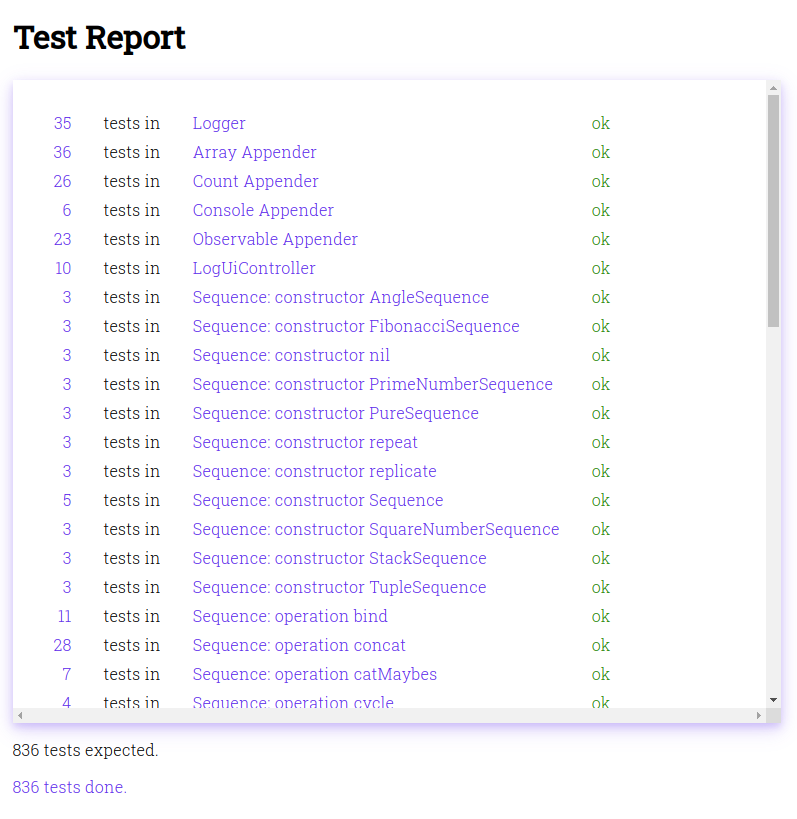
\includegraphics[width=0.8\textwidth]{mainmatter/pictures/test_report.png}
    \caption{Example Test Report}
    \label{fig:test_report}
\end{figure}


To demonstrate how to work with the test suitec, examine the following
listing~\ref{lst:testsuit_demo}:

\begin{lstlisting}[
  style=ES6, 
  caption=TestSuite demonstration,
  label={lst:testsuit_demo}
  ]
const suite = TestSuite("The truth");
suite.add("true is really true", assert => {
  assert.is(true, true);
});
suite.run();
\end{lstlisting}

Description of the functionalities: 

\begin{itemize}
  \item{|TestSuite|: A |TestSuite| contains the test cases and is identified by a
    name. This name represents the suite on the summary page on
  figure~\ref{fig:test_report}when executing.}
  \item{|run|: executes all tests containing the |TestSuite|.}
  \item{|add|: A function for including a test case into |TestStuite|. Its
      parameters are a string |name| and a callback which provides the test.}
\end{itemize}

\subsection{Additional Assertions}
\label{sub:Additional Assertions}

Assert functions in the Kolibri testing framework execute tests by comparing
two values and store the result in a summary collection of the test suite.
Listing~\ref{lst:testsuit_demo} shows the comparison of two booleans using the
|assert.is(...)| function.
This function compares an |actual| and an |expected| value. The references of
these two values must match. Otherwise, the test fails.

\subsubsection{Assertion}
\label{subsub:Assertion for Iterables}
Comparing iterables is slightly more complicated. For this reason, we extended
the testing framework with an additional assert function that compares two
arbitrary iterables. Listing~\ref{lst:iterableEq} shows the usage of this
function called |iterableEq|:

\begin{lstlisting}[
  style=ES6, 
  caption=Usage of iterableEq,
  label={lst:iterableEq}
  ]
testSuite.add("demo iterableEq", assert => {
  const sequence = Sequence(0, x => x < 2, x => x +1);

  assert.iterableEq(sequence, [0,1]);
  assert.iterableEq(sequence, Pair(0)(1));
  assert.iterableEq(sequence, Range(1));
});  
\end{lstlisting}

The implementation of |iterableEq| is suitable for any two iterables.
Listing~\ref{lst:impl_iterableEq} shows the implementation of |iterableEq|:

\begin{lstlisting}[
  style=ES6, 
  caption=Implementation of iterableEq,
  label={lst:impl_iterableEq}
  ]
// test.js
...
iterableEq: (actual, expected, maxElementsToConsume = 1_000) => { *'\label{line:signature_iterableEq}'*

    if (actual[Symbol.iterator]   === undefined) error("..."); *'\label{line:check_iterable}'*
    if (expected[Symbol.iterator] === undefined) error("...");

    const actualIt     = actual[Symbol.iterator]();
    const expectedIt   = expected[Symbol.iterator]();

    let iterationCount = 0;
    let testPassed     = true;
    let message        = "";

    while (true) {
     const { value: actualValue,   done: actualDone  } = actualIt.next();
     const { value: expectedValue, done: expectedDone } = expectedIt.next();

     const oneIteratorDone      = actualDone || expectedDone;
     const bothIteratorDone     = actualDone && expectedDone;
     const tooManyIterations    = iterationCount > maxElementsToConsume;

     //... error handling omitted ...

     iterationCount++;
    }
    if (!testPassed) error(message);
    results.push(testPassed);*'\label{line:write_result_to_summary}'*
    messages.push(message);
}
\end{lstlisting}

The implementation checks on line~\ref{line:check_iterable} if both values are
iterable. If this is the case, each value of the two iterables is compared
using a |while| loop. On line~\ref{line:write_result_to_summary}, the
test stores the result in the summary collection of the corresponding test
suite.
\newline
Since an iterable can be endless, |iterableEq| defines a default maximum
iteration amount on line~\ref{line:signature_iterableEq}.  This is handy
because it is often the case that an iterable runs infinitely when something
goes wrong. If an iterable exceeds this limit, the test fails.

\subsubsection{Assertion for Exceptions}
\label{subsub:Assertion for Exceptions}
Another extension for the testing framework is the |assert.throws| function. It
is often the case that functions must throw an exception in a specific
situation. For example, when looking for the maximum in an empty iterable.
|max| throws an exception in this case. Therefore, testing the function's
behaviour in error cases is also required. For this purpose,
listing~\ref{lst:impl_throws} shows the implementation of |assert.throws|:

\begin{lstlisting}[
  style=ES6, 
  caption=Implementation of assert.throws,
  label={lst:impl_throws}
  ]
// test.js
...
throws: (functionUnderTest, expectedErrorMsg = "") => {
     let testResult    = false;
     let message       = "";
     const hasErrorMsg = expectedErrorMsg !== "";

     try {
         functionUnderTest();*'\label{line:functionToTest}'*
         message = "Did not throw an error!";
         if (hasErrorMsg) {
             message += ` Expected: '${expectedErrorMsg}'`;
         }
         error(message);
     } catch (e) {
         testResult = true;

         if (hasErrorMsg) {
             testResult = expectedErrorMsg === e.message;
         }
     }
     results .push(testResult);
     messages.push(message);
 }
 ...
\end{lstlisting}


Line~\ref{line:functionToTest} calls the function under test. As expected, this
function should throw an exception that is caught in the catch block. If this
is the case, the test is successful. Otherwise, the test fails and a
corresponding error message is stored.

\section{Testing Table}
\label{sec:Testing Table}
This section describes the realization of the testing table. It examines the
architecture of it and how it works for a particular operation. It covers the
config-based testing approach, which enables generalizing test cases for the
Sequence library.

The architecture consists of three main parts:
\begin{itemize}
  \item{A table containing all testing functions.}
  \item{Configuration objects to define test properties.}
  \item{A function |addToTestingTable| which includes all tests from the testing
    table into a given test suite.}
\end{itemize}

Each constructor and operator of the Sequence library has its configuration
that specifies the test behavior. Likewise, each has its |TestSuite|. 

\subsection{Configuring the Testing Table}
\label{sub:Configuring the Testing Table}

In order to test operators and constructors using the testing table, it is
necessary to implement a test configuration.
Listing~\ref{lst:config_reduce} shows the testing file of the function |reduce|. 
Lines~\ref{line:start_test_config}-\ref{line:end_test_config} define the test 
configuration. Special cases not handled by the testing table follow later in
the same file from line~\ref{line:additional_test_cases} on.

\begin{lstlisting}[
  style=ES6, 
  caption=Test configuration reduce,
  label={lst:config_reduce}
  ]
const testSuite = TestSuite("Sequence: terminal operation reduce$");

addToTestingTable(testSuite)(*'\label{line:start_test_config}'*
  createTestConfig({*'\label{line:createTestConfig}'*
    name:      "reduce$",
    iterable:  () => newSequence(UPPER_SEQUENCE_BOUNDARY),
    operation: () => reduce$((acc, cur) => acc + cur, 0),
    expected:  10,
    evalFn:    expected => actual => expected === actual,
    excludedTests: [TESTS.TEST_CB_NOT_CALLED_AFTER_DONE]
  })
);*'\label{line:end_test_config}'*


testSuite.add("test: special case", assert => {*'\label{line:additional_test_cases}'*
  // Given
  // When
  // Then
});

testSuite.run();
\end{lstlisting}

On line~\ref{line:createTestConfig}, the function |createTestConfig|  sets
default values of configuration properties to simplifying the code.

The following table~\ref{tab:testing_table} shows which configuration 
properties are available and the purpose of it:

\begin{table}[H]
  \center
  \begin{tabular}{ l m{10cm} c}
    \textbf{Property} & \textbf{Description} & \textbf{Required}\\
    \hline
    |name|            & The name of the test for meaningful 
                      reporting messages. 
                    & y 
                    \\ 
    |iterable|        & A function that constructs a new iterable to apply the 
                      operation to. 
                    & y 
                    \\  
    |expected|        & The expected result of the operation applied to the iterable
                      defined in property |iterable|.
                    & 
                    y  \\ 
    |excludedTests|   & An optional array of testing function to exclude tests
                      in the testing table. 
                    & n 
                    \\
    |operation|       & The operation to test. |param| is passed as an argument
                      to it
                     (leave this empty for constructor 
                      tests since they do not take an inner iterator). 
                    & n 
                    \\
    |param|           & A parameter passed to this |operation|. If it is a
                      function, some extra tests will be performed. 
                    & n
                    \\ 
    |invariants|      & An optional array of |InvariantCallback|. The invariant 
                      must hold tests against different lists. 
                    & n
                    \\
    |evalFn|          & An optional function that takes |expected| and the |actual| 
                      in curried style. The default is |iterableEq|.
                    & n 
                    \\
  \end{tabular}
  \caption{Properties of the configuration object}
\label{tab:testing_table}
\end{table}

\subsection{The Table}
\label{sub:The Table}
The testing table is just an array (table) containing test objects.
Listing~\ref{lst:testing_table} shows the implementation.

\begin{lstlisting}[
  style=ES6, 
  caption=Testing Table,
  label={lst:testing_table}
  ]
const testingTable = [
  { name: TESTS.TEST_SIMPLE,                   test: testSimple},
  { name: TESTS.TEST_PURITY,                   test: testPurity},
  { name: TESTS.TEST_CB_NOT_CALLED_AFTER_DONE, test: testCBNotCalledAfterDone},
  { name: TESTS.TEST_PROTOTYPE,                test: testPrototype},
  { name: TESTS.TEST_INVARIANTS,               test: testInvariants},
  { name: TESTS.TEST_ITERATE_MULTIPLE_TIMES,   test: testIterateMultipleTimes},
];
\end{lstlisting}

An object in the table includes two properties:
\begin{itemize}
\item{A string representing its name. The name is important for displaying an accurate error message if the test fails.}
\item{A function to test a specific behavior}
\end{itemize}

Each function of the testing table expects as argument a test configuration
object of type |SequenceTestConfigType|. Listing~\ref{lst:test_simple} presents
exemplary the implementation of |testSimple|.

\begin{lstlisting}[
  style=ES6, 
  caption=Implementaion Test Simple,
  label={lst:test_simple}
  ]
/**
 * @type {
 *             (config: SequenceTestConfigType)
 *          => (assert: AssertType)
 *          => void
 *       }
 */
const testSimple = config => assert => {
  const { iterable, operation, evalFn, expected, param } = config;*'\label{line:test_config_destructuring}'*
  const baseIterable = iterable(); *'\label{line:test_config_iterable}'*
  const operated     = operation(param)(baseIterable);*'\label{line:test_config_operated}'*
  evaluate(expected, operated, assert, evalFn);*'\label{line:test_config_eval}'*
};
\end{lstlisting}

The function |simpleTest| examines whether an operation correctly processes a typical use case.
For this purpose, it executes the following tasks: 
\begin{itemize}
  \item{Line~\ref{line:test_config_iterable} shows the invocation of the
      function |iterable| to create an iterable for further use.}
  \item{Line~\ref{line:test_config_operated} executes the operation to test on
      the previously obtained iterable by passing the required parameters.
      |param| is optional and can, therefore, also be left empty. This covers
      cases where operations need to be parametrized (like |map|, which takes a
      mapping function).}
  \item{Line~\ref{line:test_config_eval} calls a function |evaluate|, which
      then calls the passed function |evalFn|, comparing the |actual| and
      |expected| values. This gives the possibility to evaluate iterables or
      sequences containing more complex values or if the output of an operation
      is not an iterable anymore (as, for example, |reduce|). If |evalFn| is
    undefined, the fallback function |iterableEq| is used, comparing two
  iterables as section~\ref{sub:Additional Assertions} explains.} 
\end{itemize}

The testing table includes test-functions to examine the following behaviors of
implementations of the Sequence library:

\begin{itemize}
  \item{\textbf{testSimple} checks if a typical case works properly.}
  \item{\textbf{testPurity} checks if an operator makes some side effects.}
  \item{\textbf{testCBNotCalledAfterDone} checks if a given callback of an
    operator will be called when the Iterable is exhausted.}
  \item{\textbf{testPrototype} checks if the |SequencePrototype| is set.}
  \item{\textbf{testInvariants} checks if an invariant holds by applying different parameters.}
  \item{\textbf{testIterateMultipleTimes} checks if an iterable produces the same output twice.}
\end{itemize}

\subsection{Running the Testing Table}
\label{sub:Running the Testing Table}
|addToTestingTable| must be called for each configuration to be tested by the
testing table. It runs each test with the given configuration
(line~\ref{line:add_to_testsuite}). Some tests do not make sense for all
functions of the Sequence library - since |addToTestingTable| runs all tests by
default, it must provide an option to exclude such tests. For
example, if an operation has no callback, the check of its side effect is
useless.

Line~\ref{line:filtering_tests} filters out tests excluded by the
configuration. 
\begin{lstlisting}[
  style=ES6, 
  caption=The addToTestingTable function,
  label={lst:impl_addToTestingTable}
  ]
export { addToTestingTable }
...
/**
 * @type {
 *       (testSuite: TestSuiteType)
 *    => (config: SequenceTestConfigType)
 *    => void
 * }
 */
const addToTestingTable = testSuite => config => {
  const { excludedTests } = config;

  testingFunctions
    .filter (({ name })        => !excludedTests.includes(name)) *'\label{line:filtering_tests}'*
    .forEach(({ name, test })  => 
         testSuite.add(`${name}: ${config.name}`, test(config)));*'\label{line:add_to_testsuite}'*
};
\end{lstlisting}


\section{Testing based on Properties}
\label{sec:Testing based on Properties}
John Huges and Carl Claessen wrote to following sentence in the paper
"Quickcheck, A Lighweight Tool for Random Testing of Haskell Programms":
\textit{
Despite anecdotal evidence that functional programs require somewhat less
testing (`Once it type-checks, it usually works'), in practice it is still a 
major part of functional program development}~\cite{quickcheck_hughes}.
If these programming icons claim it takes many tests even in a strongly typed 
language, how many does it take in JavaScript? Of course, enough.

\subsection{Invariant Testing}
\label{sub:Invariant Testing}
Invariant tests add another layer of verification to ensure the correctness of
the Sequence library. Some aspects of this testing are leaned on the Quickcheck
approach of the paper mentioned before. We concentrated on only some essential
parts since implementing the whole Quickcheck framework would compared to the
effort not bring enough benefits for this work.
\newline
The test configuration object contains a property |invariant|. It allows
defining of some invariants, which are tested against different iterables.
Quickcheck does this with randomly generated data. Our data is fixed and
includes a mix of special cases.
\newline
Line~\ref{line:reverse_law} in listing~\ref{lst:test_config_reverse} defines
the invariants of |reverse|. This statement defines that an iterable must be 
equal to the original when reversed two times.

\begin{lstlisting}[
  style=ES6, 
  caption=Test Configuration reverse,
  label={lst:test_config_reverse}
  ]
const testSuite = TestSuite("Sequence: operation reverse$");

addToTestingTable(testSuite)(
  createTestConfig({
    name:      "reverse$",
    iterable:  () => newSequence(UPPER_SEQUENCE_BOUNDARY),
    operation: () => reverse$,
    expected:  [4, 3, 2, 1, 0],
    invariants: [
      *'\colorbox{code-highlight}{it => reverse$(reverse$(it)) ["=="] (it), }'* *'\label{line:reverse_law}'*
    ]
  })
);

testSuite.run();
\end{lstlisting}
The testing table contains a test function |testInvariants|.
Listing~\ref{lst:invariant_penetration} defines that function:

\begin{lstlisting}[
  style=ES6, 
  caption=Implementation invariant penetration,
  label={lst:invariant_penetration}
  ]
/**
 * Applies a series of lists to a given invariant.
 * @template _T_
 * @type {
 *            (invariants: InvariantCallback)
 *         => (assert: AssertType)
 *         => void
 *       }
 */
const invariantPenetration = invariant => assert => {
  const testingLists = [ *'\label{line:list_of_parameters}'*
    // edge case
    nil,                                                   
    // edge case, done calculated
    newSequence(1),                                        
    // typical number
    newSequence(3),                                        

    // no big iterable, needs extra test

    // edge case, done set explicitly
    PureSequence("testString"),                            
    // mixing types
    ['a', 'b', 'c', 1, 2, 3, Nothing, Just("testString")], 
    // iterable of iterables
    [PureSequence(1), newSequence(4), '#', "abc", 1]       
  ];

  for (const list of testingLists) {
    const result = invariant(list);
    assert.isTrue(result);
  }
};
\end{lstlisting}

Line~\ref{line:list_of_parameters} defines a list with several parameters of
type |Iterable|. Each parameter tests if the invariant of |reverse| holds. 
This enables for testing many cases written in a few lines of code.

\subsubsection{An advanced Example}
\label{subsub:An advanced Example}
|mconcat| is an operation to flatten an iterable of iterables. If |mconcat|
follows certain laws, the sequence forms a monoid under this
operation.~\cite{haskell_monoid}
Listing~\ref{lst:lr_identity_mconcat} shows the definition of the identity law
for the function |<>| in Haskell which concatenates two lists:

\begin{lstlisting}[
  style=Haskell,
  caption=Left and right identity of <> in Haskell,
  label={lst:lr_identity_mconcat}
]
-- left identity
x <> mempty = x
-- right identity
mempty <> x = x
\end{lstlisting}

The |<>| operator is defined on the semigroup, a monoid subset.
Listing~\ref{lst:lr_identity_mconcat} demonstrates that a list $x$ concatenated
with |nil|, the empty list, equals the original one. As |<>|, |mconcat| is also
associative and a concatenation with the neutral element (the empty sequence)
has no influence on the result.\\ 
With the previously shown implementation of the invariant based testing, it
becomes possible to test these laws for |mconcat|!
Listing~\ref{lst:mconcat_invariant} shows the implementation of these
invariants in JavaScript:

\begin{lstlisting}[
  style=ES6, 
  caption=Invariants of mconcat,
  label={lst:mconcat_invariant}
  ]
addToTestingTable(testSuite)(
  createTestConfig({
    name:       "mconcat",
    iterable:   () => 
      toMonadicIterable([ newSequence(2), newSequence(2), newSequence(2) ]),
    operation:  () => mconcat,
    expected:   [0, 1, 2, 0, 1, 2, 0, 1, 2],
    invariants: [
      it => mconcat([nil, it]) ["=="] (it),*'\label{line:mconcat_first_invariant}'*
      it => mconcat([it, nil]) ["=="] (it),*'\label{line:mconcat_second_invariant}'*
      it => [...mconcat([PureSequence(1),it])].length > [...it].length,
    ],
  })
)
\end{lstlisting}

Let us focus on line~\ref{line:mconcat_first_invariant} and 
\ref{line:mconcat_second_invariant}.
The property |invariants| expect an array of functions. Each of these
functions represents a law. Therefore, the function injects an arbitrary
iterable called |it|, and the law must hold for it.

\subsection{Revealed Code Bugs: Discoveries through Testing during Development}
\label{sub:Revealed Code Bugs: Discoveries through Testing during Development}
As illustrated in the testing table section, a test case named
|TEST_CB_NOT_CALLED_AFTER_DONE| guarantees that a callback is not invoked once
an iterator is exhausted. This test arose from a bug during development
that it is expected for a callback not to be called after the iterator is used
up. Such occurrences could lead to program errors or unexpected behaviour.
Consequently, we implemented a test case addressing this scenario and added it
to the testing table. By adding just one more test, the entire Sequence library
could be examined for this behaviour, allowing for further improvements and
finding the same bug in other functions!
\\
Another example concerns the behaviour of operators and operations when dealing
with empty iterables. As soon as a test configuration provides an invariant,
this test runs against the empty sequence.\\
Furthermore, another special test case is the |TEST_PURITY|, which ensures that
the state of an iterable is in the proper location. This safeguards against
unexpected side effects, promoting a more reliable program execution.

\subsection{Conclusion}
\label{sub:Conclusion}
When implementing large code bases, having a solid test framework is crucial.
Structured extension of the test suite during development leads to extensive
core functionality testing. Thus, the core becomes even more robust when the
code base grows!
\newline
The standardization and generalization of tests using a testing table imply that
writing tests for new functionalities takes less time and ensures better
quality.

\input{./mainmatter/development/naming}
% chapter development (end)
